%%%%%%%%%%%%%%%%%%%%%%%%%%%%%%%%%%%%%%%%%
% Beamer Presentation
% LaTeX Template
% Version 1.0 (10/11/12)
%
% This template has been downloaded from:
% http://www.LaTeXTemplates.com
%
% License:
% CC BY-NC-SA 3.0 (http://creativecommons.org/licenses/by-nc-sa/3.0/)
%
%%%%%%%%%%%%%%%%%%%%%%%%%%%%%%%%%%%%%%%%%

%----------------------------------------------------------------------------------------
%	PACKAGES AND THEMES
%----------------------------------------------------------------------------------------

\documentclass[aspectratio=169]{beamer}
\usepackage[portuges]{babel}
\usepackage[utf8]{inputenc}
\usepackage[alf]{abntex2cite}	
\usepackage[portuguese, linesnumbered, vlined, titlenumbered, ruled]{algorithm2e}
\usepackage{algpseudocode}
\usepackage{beamerthemesplit}
\usepackage{multirow}
\usepackage{scalefnt}
\usepackage{enumerate}

% Macro que faz com que a numeracao de diferentes algoritmos continue de onde parou
\newcommand{\rememberlines}{\xdef\rememberedlines{\number\value{AlgoLine}}}
\newcommand{\resumenumbering}{\setcounter{AlgoLine}{\rememberedlines}}

% The Beamer class comes with a number of default slide themes
% which change the colors and layouts of slides. Below this is a list
% of all the themes, uncomment each in turn to see what they look like.

%\usetheme{default}
%\usetheme{AnnArbor}
%\usetheme{Antibes}
%\usetheme{Bergen}
%\usetheme{Berkeley}
%\usetheme{Berlin}
%\usetheme{Boadilla}
%\usetheme{CambridgeUS}
%\usetheme{Copenhagen}
%\usetheme{Darmstadt}
%\usetheme{Dresden}
%\usetheme{Frankfurt}
%\usetheme{Goettingen}
%\usetheme{Hannover}
%\usetheme{Ilmenau}
%\usetheme{JuanLesPins}
%\usetheme{Luebeck}
\usetheme{Madrid}
%\usetheme{Malmoe}
%\usetheme{Marburg}
%\usetheme{Montpellier}
%\usetheme{PaloAlto}
%\usetheme{Pittsburgh}
%\usetheme{Rochester}
%\usetheme{Singapore}
%\usetheme{Szeged}
%\usetheme{Warsaw}

% As well as themes, the Beamer class has a number of color themes
% for any slide theme. Uncomment each of these in turn to see how it
% changes the colors of your current slide theme.

%\usecolortheme{albatross}
%\usecolortheme{beaver}
%\usecolortheme{beetle}
%\usecolortheme{crane}
\usecolortheme{dolphin}
%\usecolortheme{dove}
%\usecolortheme{fly}
%\usecolortheme{lily}
%\usecolortheme{orchid}
%\usecolortheme{rose}
%\usecolortheme{seagull}
%\usecolortheme{seahorse}
%\usecolortheme{whale}
%\usecolortheme{wolverine}

%\setbeamertemplate{footline} % To remove the footer line in all slides uncomment this line
%\setbeamertemplate{footline}[page number] % To replace the footer line in all slides with a simple slide count uncomment this line

%\setbeamertemplate{navigation symbols}{} % To remove the navigation symbols from the bottom of all slides uncomment this line


\usepackage{graphicx} % Allows including images
\usepackage{booktabs} % Allows the use of \toprule, \midrule and \bottomrule in tables

%----------------------------------------------------------------------------------------
%	TITLE PAGE
%----------------------------------------------------------------------------------------

\title[Árvores AVL]{Algoritmos e Estrutura de Dados}
\subtitle{Árvores AVL}
\author[Frederico Santos de Oliveira]{prof. Frederico Santos de Oliveira}
\institute[UFMT]{Universidade Federal de Mato Grosso\\ Faculdade de Engenharia}
\date{}

\begin{document}

%------------------------------------------------
\begin{frame}
\titlepage % Print the title page as the first slide

\begin{figure}[!h]
  \centering
   
\includegraphics[width=120pt]{imagens/balanca.jpg}
  \label{fig_introducao}
\end{figure}
\end{frame}

%------------------------------------------------

\begin{frame}
\frametitle{Roteiro} % Table of contents slide, comment this block out to remove it
\tableofcontents % Throughout your presentation, if you choose to use \section{} and \subsection{} commands, these will automatically be printed on this slide as an overview of your presentation
\end{frame}

%----------------------------------------------------------------------------------------
%	PRESENTATION SLIDES
%----------------------------------------------------------------------------------------

%------------------------------------------------
\section{Objetivos}

\begin{frame}
\frametitle{Objetivos}
Esta aula tem como objetivos:
\begin{enumerate}
\item Apresentar os conceitos básicos sobre árvores balanceadas AVL;
\item Demonstrar os algoritmos por meio de pseudo-códigos.
\end{enumerate}
\end{frame}

%------------------------------------------------
% 
% \section{Referências bibliográficas}
%   \frame{\frametitle{Referências bibliográficas}
%     \bibliographystyle{abntex2-alf}
%     \bibliography{referencias}
%   }
%   
%------------------------------------------------
\section{Introdução} % Sections can be created in order to organize your presentation into discrete blocks, all sections and subsections are automatically printed in the table of contents as an overview of the talk
%------------------------------------------------

\begin{frame}
\frametitle{Introdução}
\begin{itemize}
 \item As árvores balanceadas foram introduzidas em 1962 por {\bf Adelson-Velskii e Landis}, daí o nome {\bf Árvores AVL}.
 \item As operações de busca, inserção e remoção em uma árvore com $n$ elementos podem ser efetuadas em O($\log_2n$), mesmo no pior caso.
 \item Os autores garantem que a árvore balanceada nunca será 45\% mais alta que a árvore perfeitamente balanceada correspondente, independentemente do número de nós existentes
\end{itemize}
\end{frame}

%------------------------------------------------

\begin{frame}{Introdução}{Árvore Balanceada}
\begin{figure}[!h]
  \centering
   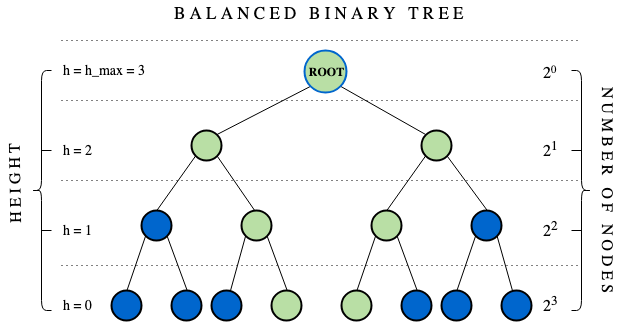
\includegraphics[width=150pt]{imagens/balanced_tree.png}
  \label{fig_balanced_tree}
\end{figure}
\end{frame}


%------------------------------------------------

\begin{frame}{Introdução}{Árvore Balanceada x Árvore Degenerada}
\begin{figure}[!h]
  \centering
   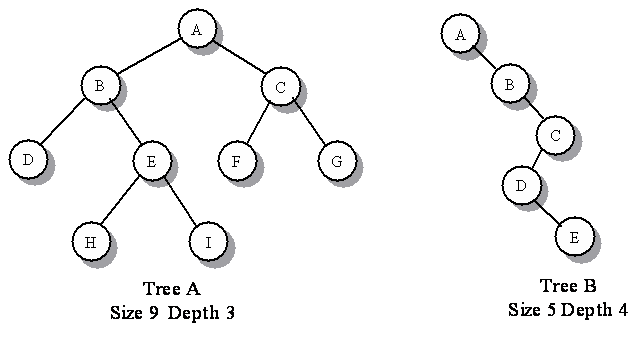
\includegraphics[width=150pt]{imagens/degenerated_tree.png}
  \label{fig_degenerated_tre}
\end{figure}
\end{frame}


%------------------------------------------------

\begin{frame}{Introdução}{Fator de Balanceamento}
\begin{figure}[!h]
  \centering
   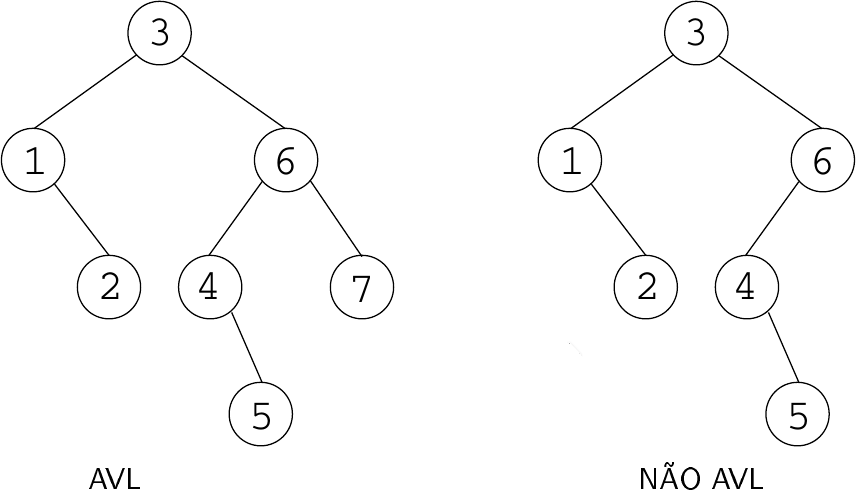
\includegraphics[width=250pt]{imagens/exemplo_avl.png}
  \label{fig_exemplo_avl}
\end{figure}
\end{frame}

%------------------------------------------------

\begin{frame}
\frametitle{Introdução}
\begin{itemize}
 \item Uma árvore AVL é definida como:
\begin{itemize}
\item Uma árvore vazia, ou
\item Uma Árvore Binária de Busca $T$ cujas subárvores esquerda e direita, denominadas respectivamente $L$ e $R$, satisfaçam as condições:
\begin{itemize}
\item $L$ e $R$ são árvores AVL.
\item $|h_L - h_R| \leq$ 1, onde $h_L$ e $h_R$ são as alturas das subárvores $L$ e $R$, respectivamente
\end{itemize}
\end{itemize}
\item A definição de uma Árvore AVL requer que cada subárvore seja também de altura equilibrada.
\end{itemize}
\end{frame}

%------------------------------------------------
\subsection{Altura}
%------------------------------------------------

\begin{frame}{Introdução}{Altura de um nodo}
A altura de um nodo é calculada da seguinte forma:
 \begin{itemize}
 \item Verifica se o nodo é um nodo folha. 
 \begin{itemize}
 \item Caso sim, sua altura é zero.
 \begin{itemize}
 \item Por convenção, se o nodo folha possui altura zero, seus filhos (NULL) possuem altura -1.
 \end{itemize}
 \item Caso contrário, obtém-se a maior altura entre suas subárvores, adicionando um.
 \end{itemize} 
 \end{itemize} 
A seguir, o pseudocódigo. 
\end{frame}

%------------------------------------------------

\begin{frame}{Introdução}{Altura de um nodo}
% \scalebox{0.5}{
\begin{algorithm}[H]
\caption{CalculaAltura} 
\label{CalculaAltura}
\Entrada{Ponteiro para o nodo $r$.}
\Saida{Altura do nodo $r$.}
\Inicio{
  \Se {(r = NULL)} {
    \Retorna { -1}
  }
  \Senao {
    alt\_esq $\leftarrow$ AlturaNodo($r$.esq) \\
    alt\_dir $\leftarrow$ AlturaNodo($r$.dir) \\
    \Se {(alt\_esq $>$ alt\_dir)} {
      \Retorna alt\_esq + 1
    }
    \Senao {
      \Retorna alt\_dir + 1
    }
  }
}
\end{algorithm}
% }
\tiny{Adaptado de \cite{Backes2016}}    
\end{frame}

%------------------------------------------------

\begin{frame}{Introdução}{Altura de um nodo}
\begin{itemize}
 \item Calcular a altura de um nodo tem custo $O(\log_2n)$, que é a altura de uma árvore AVL.
 \item A altura será atualizada apenas após inserções e remoções.
 \item A fim de minimizar esse custo, armazena-se a altura no nodo e atualiza apenas quando necessário.
 \item Portanto, deve-se calcular a altura de cada nodo.
\end{itemize}
\end{frame}

%------------------------------------------------

\begin{frame}{Introdução}{Altura de um nodo}
% \scalebox{0.8}{
\begin{algorithm}[H]
\caption{AlturaNodo} 
\label{AlturaNodo}
\Entrada{Ponteiro para o nodo $n$.}
\Saida{Altura do nodo $n$.}
\Inicio{
  \Se {(n = NULL)} {
    \Retorna ( -1  )
  }
  \Senao {
    \Retorna n.altura
  }
}
\end{algorithm}
% }  
\tiny{Adaptado de \cite{Backes2016}}  
\end{frame}

%------------------------------------------------
\section{Fator de Balanceamento}
%------------------------------------------------

\begin{frame}{Introdução}{Fator de Balanceamento}
\begin{itemize}
 \item O fator de balanceamento (FB) de um nodo $T$ é definido como sendo $h_L - h_R$, em que $h_L$ e $h_R$ são as alturas das subárvores esquerda e direita de $T$, respectivamente
 \item Para qualquer nó $T$ em uma árvore AVL, o FB assume o valor -1, 0 ou +1
 \item Um nodo folha possui FB igual a zero.
\end{itemize}
\end{frame}

%------------------------------------------------

\begin{frame}{Introdução}{Fator de Balanceamento}
\begin{figure}[!h]
  \centering
   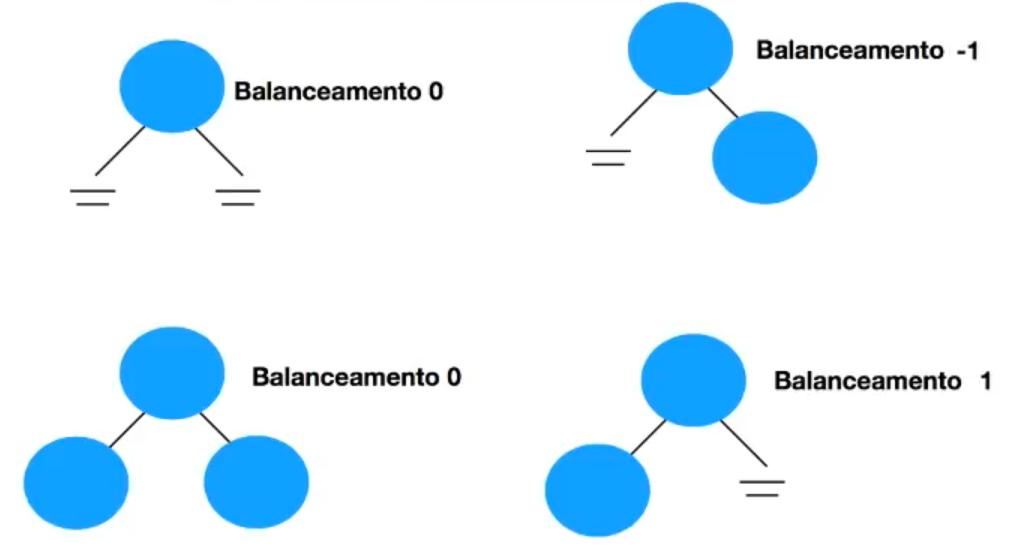
\includegraphics[width=200pt]{imagens/balanceamento.png}
  \label{fig_balanced_tree}
\end{figure}
\end{frame}

%------------------------------------------------

\begin{frame}{Introdução}{Fator de Balanceamento}
\begin{figure}[!h]
  \centering
   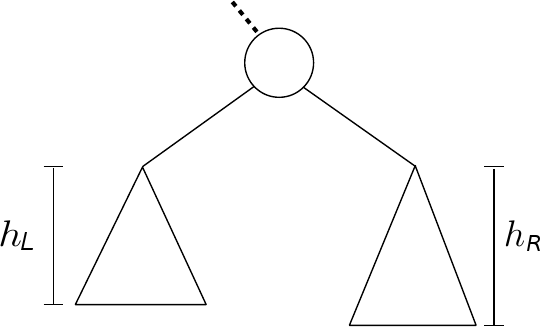
\includegraphics[width=150pt]{imagens/alturas_subarvores.png}
  \label{fig_alturas_subarvores}
\end{figure}
\end{frame}

%------------------------------------------------

\begin{frame}{Introdução}{Fator de Balanceamento}
\begin{figure}[!h]
  \centering
   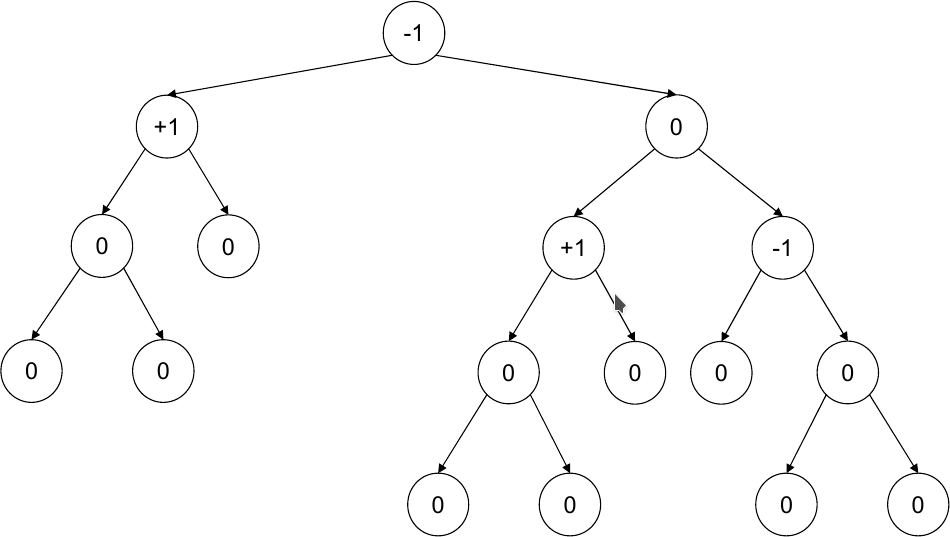
\includegraphics[width=250pt]{imagens/fator_balanceamento.png}
  \label{fig_fator_balanceamento}
\end{figure}
\end{frame}

%------------------------------------------------

\begin{frame}{Introdução}{Fator de Balanceamento}
\begin{figure}[!h]
  \centering
   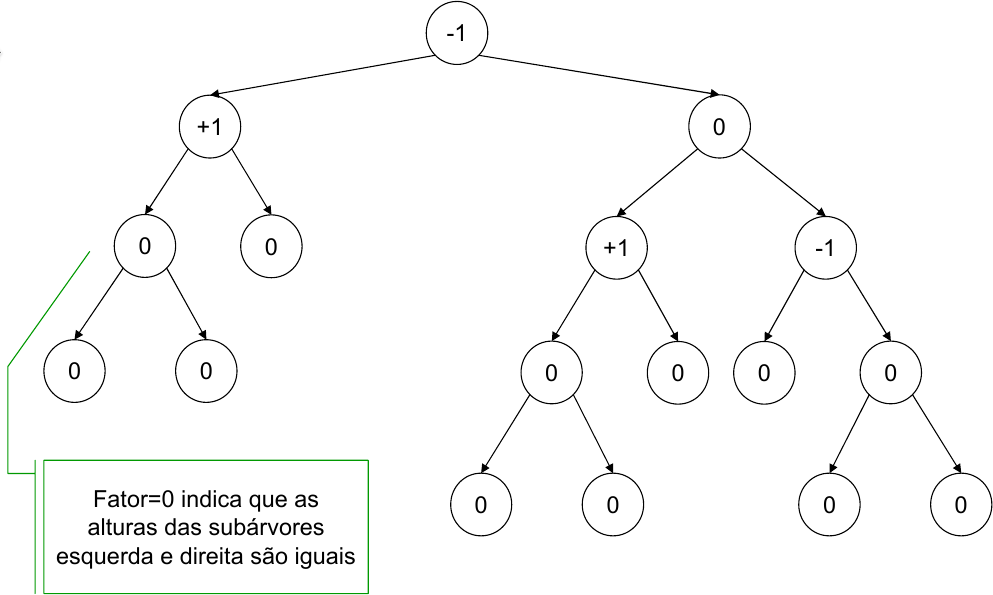
\includegraphics[width=250pt]{imagens/fator_balanceamento1.png}
  \label{fig_fator_balanceamento1}
\end{figure}
\end{frame}

%------------------------------------------------

\begin{frame}{Introdução}{Fator de Balanceamento}
\begin{figure}[!h]
  \centering
   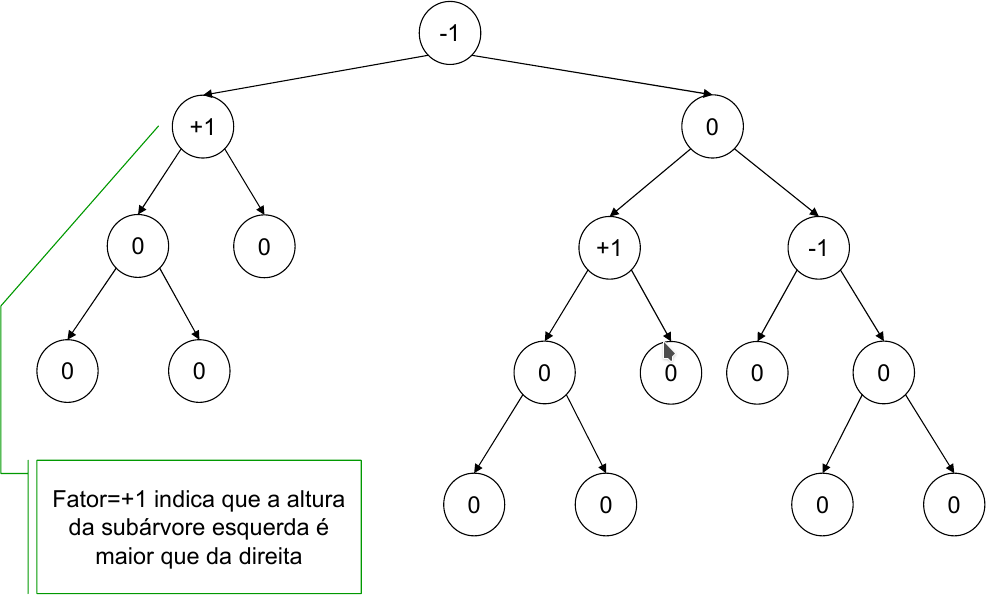
\includegraphics[width=250pt]{imagens/fator_balanceamento2.png}
  \label{fig_fator_balanceamento2}
\end{figure}
\end{frame}

%------------------------------------------------

\begin{frame}{Introdução}{Fator de Balanceamento}
\begin{figure}[!h]
  \centering
   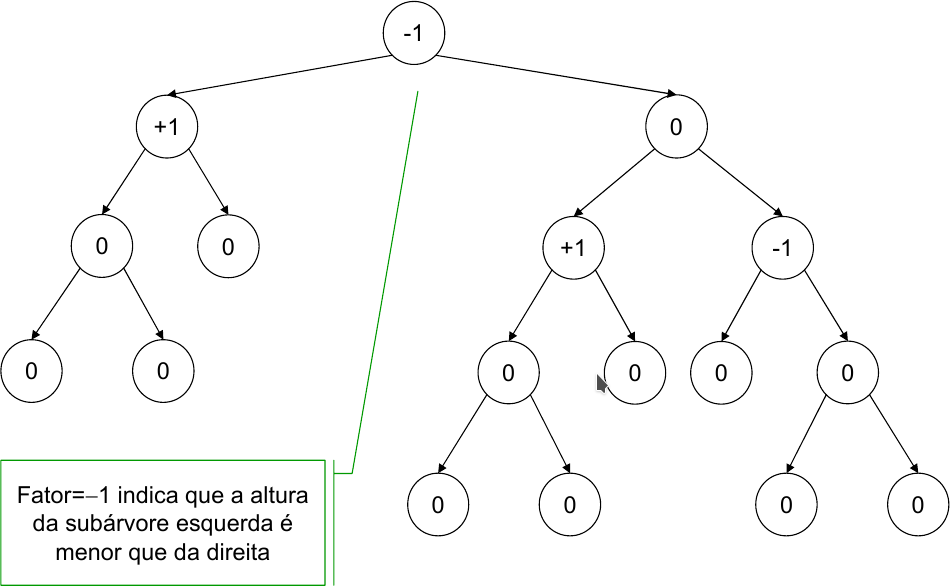
\includegraphics[width=250pt]{imagens/fator_balanceamento3.png}
  \label{fig_fator_balanceamento3}
\end{figure}
\end{frame}

%------------------------------------------------

\begin{frame}{Introdução}{Fator de Balanceamento}
\begin{algorithm}[H]
\caption{FatorBalanceamento} 
\label{FatorBalanceamento}
\Entrada{Ponteiro para o nodo $n$.}
\Inicio{
  \Retorna abs(AlturaNodo(n.esq) - AlturaNodo(n.dir))
}
\end{algorithm}
\end{frame}

%------------------------------------------------
\section{Rotações}
%------------------------------------------------

\begin{frame}{Introdução}{Rotações}
\begin{itemize}
 \item O processo de rebalanceamento é conduzido utilizando 4 tipos de rotações: 
 \begin{itemize}
 \item 2 Rotações Simples:
 \begin{itemize}
 \item Rotação Simples à Direita (denominada Rotação LL).
 \item Rotação Simples à Esquerda (denominada Rotação RR). 
 \end{itemize}
 \item 2 Rotações Duplas:
 \begin{itemize}
 \item Rotação Dupla à Esquerda e à Direita (denominada Rotação RL).
 \item Rotação Dupla à Direita e à Esquerda (denominada Rotação LR).
 \end{itemize} 
 \end{itemize}
  \item As rotação LL e RR são simétricas entre si assim como LR e RL.
\end{itemize}
\end{frame}

%------------------------------------------------
\subsection{Rotação LL}
%------------------------------------------------

\begin{frame}{Rotação LL}
\begin{figure}[!h]
  \centering
   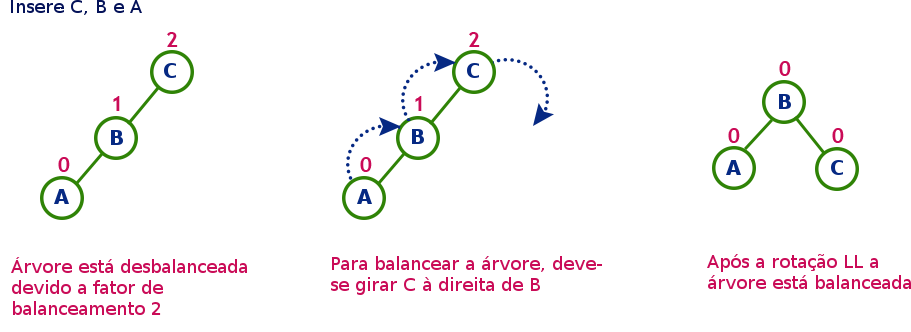
\includegraphics[width=300pt]{imagens/rotacao_ll.png}
  \label{fig_rotacao_ll}
\end{figure}
\end{frame}

%------------------------------------------------

\begin{frame}{Rotação LL}
\begin{figure}[!h]
  \centering
  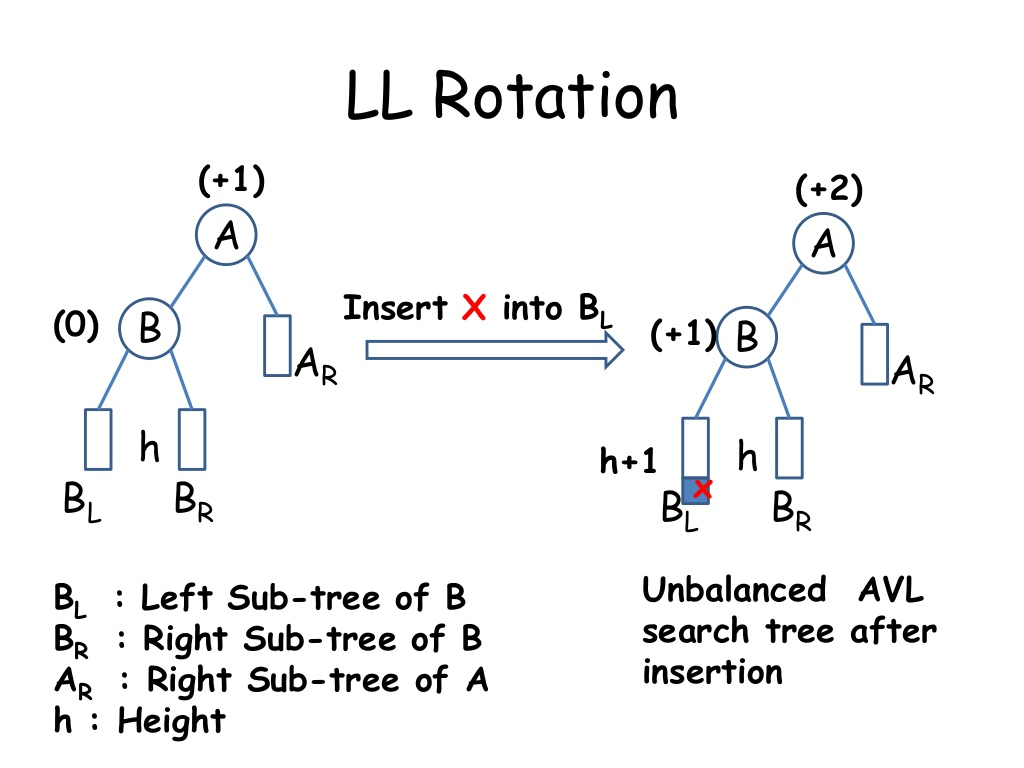
\includegraphics[width=300pt]{imagens/ll_rotation.png}
  \label{fig_ll_rotation}
\end{figure}
\end{frame}

%------------------------------------------------

\begin{frame}{Rotação LL}
\begin{figure}[!h]
  \centering
  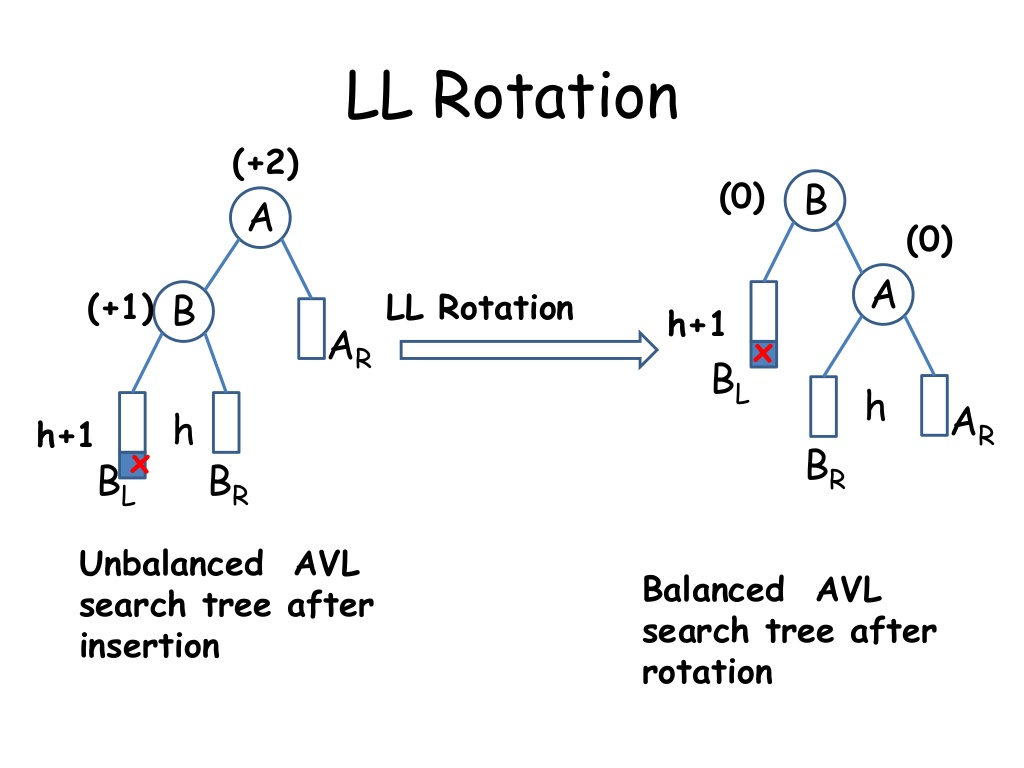
\includegraphics[width=300pt]{imagens/ll_rotation1.png}
  \label{fig_ll_rotation1}
\end{figure}
\end{frame}

%------------------------------------------------

\begin{frame}{Rotação LL}{Exemplo}
\begin{figure}[!h]
  \centering
  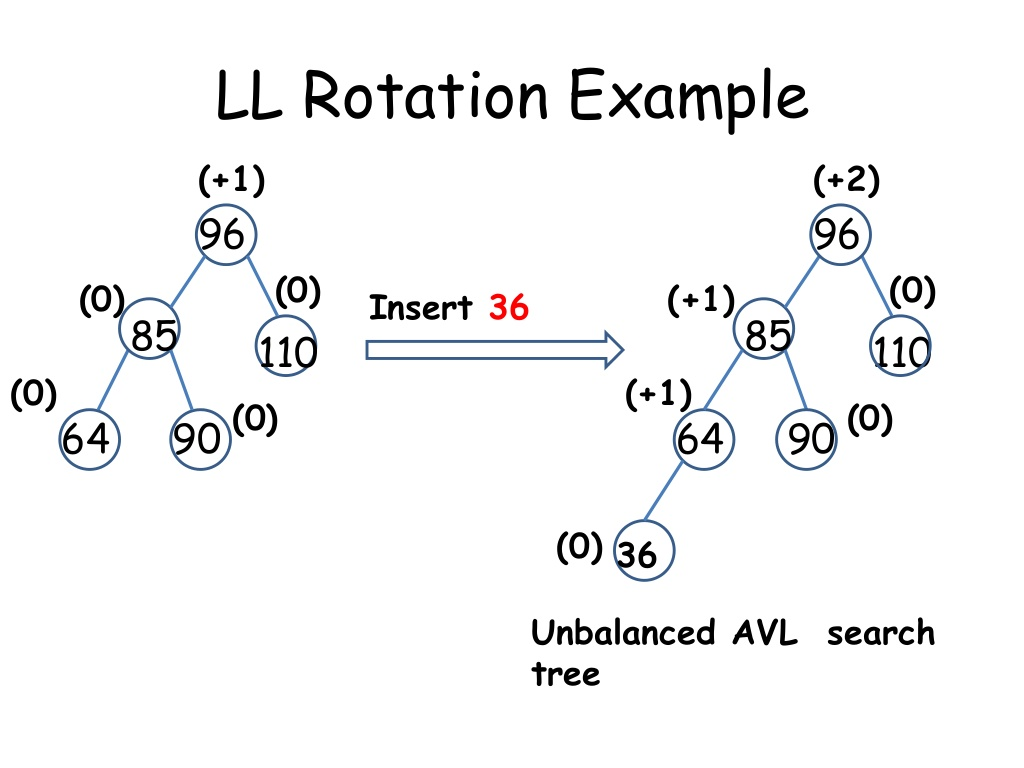
\includegraphics[width=300pt]{imagens/ll_rotation_example.png}
  \label{fig_ll_rotation_example}
\end{figure}
\end{frame}

%------------------------------------------------

\begin{frame}{Rotação LL}{Exemplo}
\begin{figure}[!h]
  \centering
  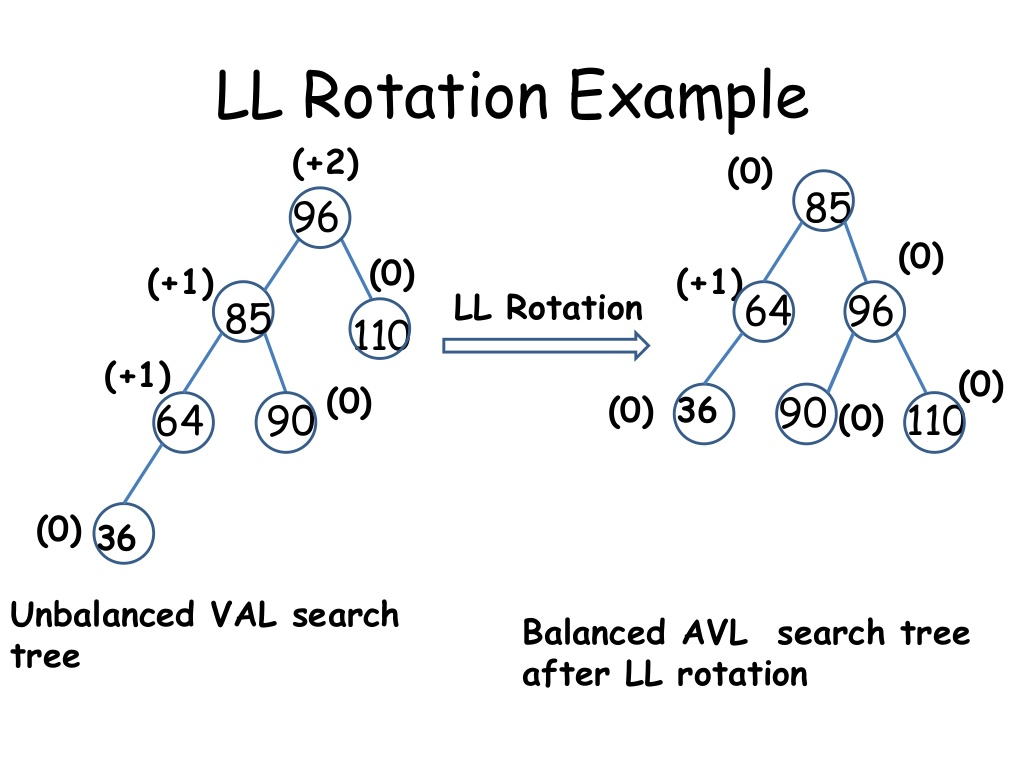
\includegraphics[width=300pt]{imagens/ll_rotation_example1.png}
  \label{fig_ll_rotation_example1}
\end{figure}
\end{frame}
%------------------------------------------------

\begin{frame}{Rotação LL}
% \scalebox{0.8}{
\begin{algorithm}[H]
\caption{RotaçãoLL} 
\label{RotacaoLL}
\Entrada{Ponteiro para o nodo desbalanceado $A$.}
\Inicio{
  B $\leftarrow$ A.esq \\
  A.esq $\leftarrow$ B.dir \\
  B.dir $\leftarrow$ A \\
  A.altura $\leftarrow$ maior(AlturaNodo(A.esq), AlturaNodo(A.dir)) + 1 \\
  B.altura $\leftarrow$ maior(AlturaNodo(B.esq), A.altura) + 1 \\
  A $\leftarrow$ B \\
}
\end{algorithm}
% }  
\tiny{Adaptado de \cite{Backes2016}}  
\end{frame}

%------------------------------------------------
\subsection{Rotação RR}
%------------------------------------------------

\begin{frame}{Rotação RR}
\begin{figure}[!h]
  \centering
   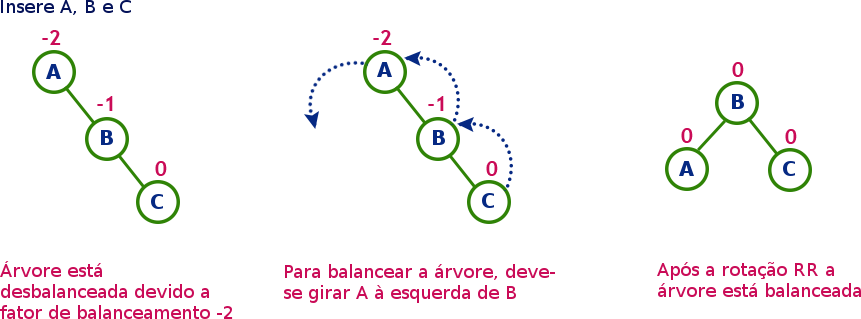
\includegraphics[width=300pt]{imagens/rotacao_rr.png}
  \label{fig_rotacao_rr}
\end{figure}
\end{frame}

%------------------------------------------------

\begin{frame}{Rotação RR}
\begin{figure}[!h]
  \centering
  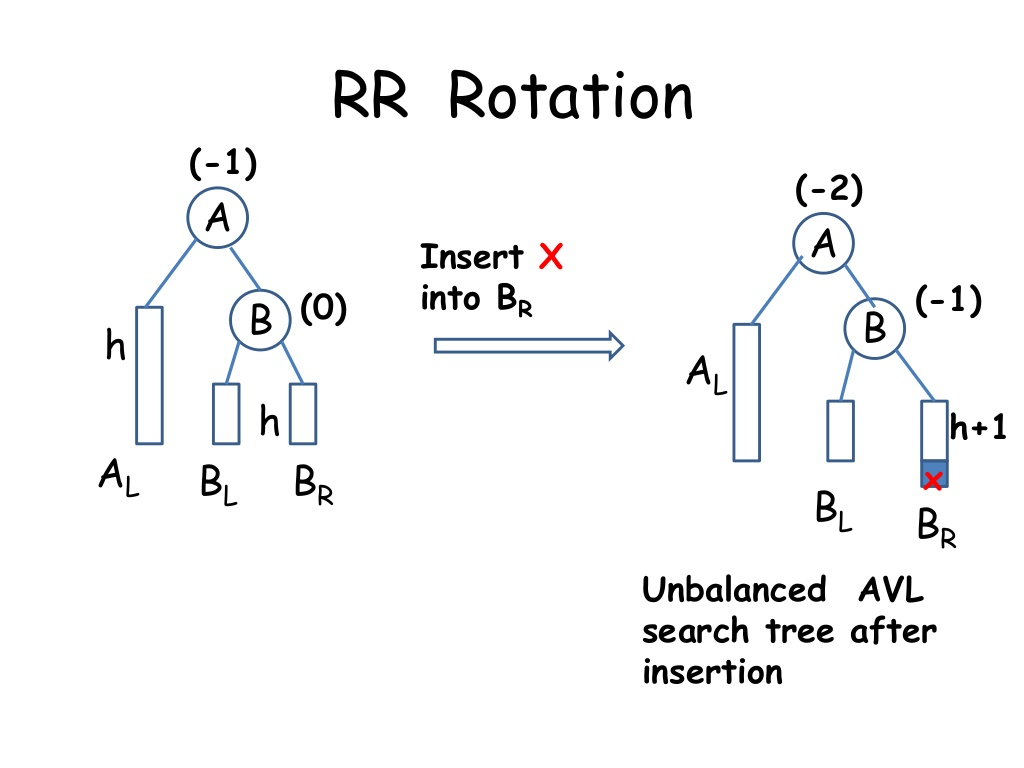
\includegraphics[width=300pt]{imagens/rr_rotation.png}
  \label{fig_rr_rotation}
\end{figure}
\end{frame}

%------------------------------------------------

\begin{frame}{Rotação RR}
\begin{figure}[!h]
  \centering
  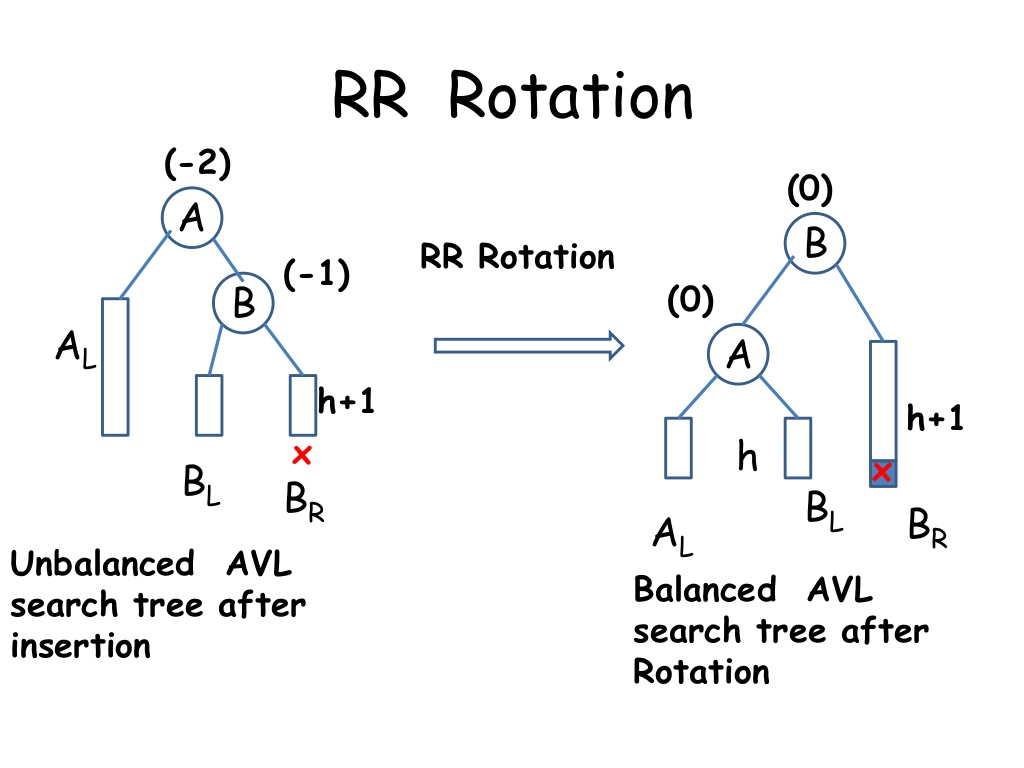
\includegraphics[width=300pt]{imagens/rr_rotation1.png}
  \label{fig_rr_rotation1}
\end{figure}
\end{frame}

%------------------------------------------------

\begin{frame}{Rotação RR}{Exemplo}
\begin{figure}[!h]
  \centering
  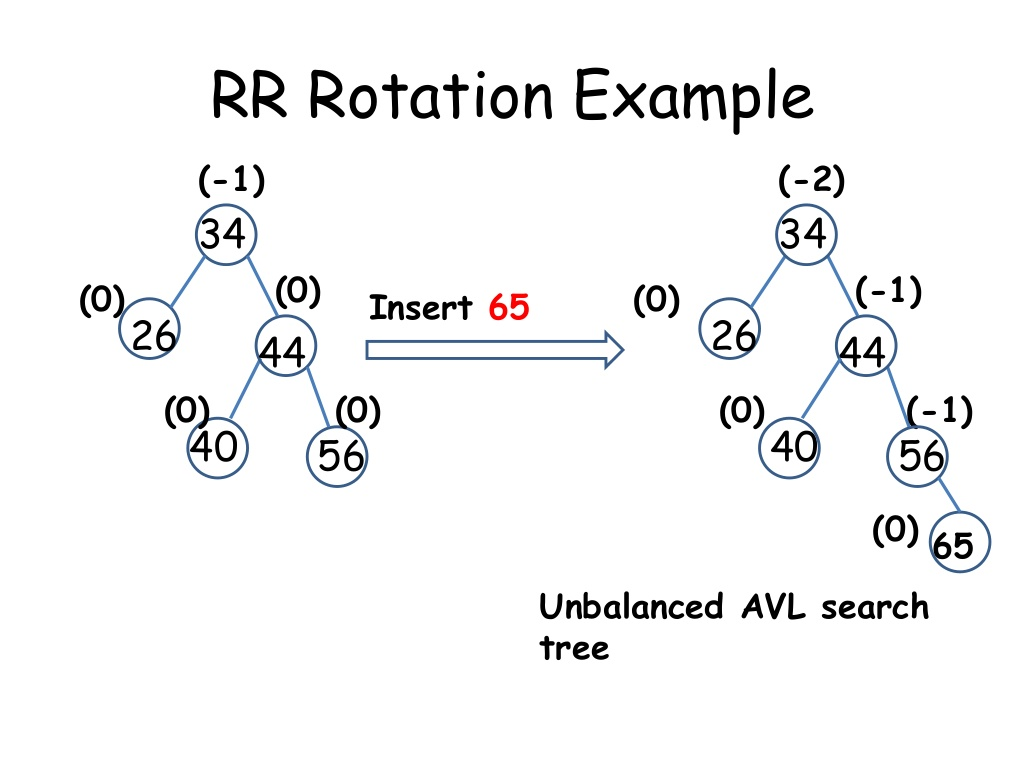
\includegraphics[width=300pt]{imagens/rr_rotation_example.png}
  \label{fig_rr_rotation_example}
\end{figure}
\end{frame}

%------------------------------------------------

\begin{frame}{Rotação RR}{Exemplo}
\begin{figure}[!h]
  \centering
  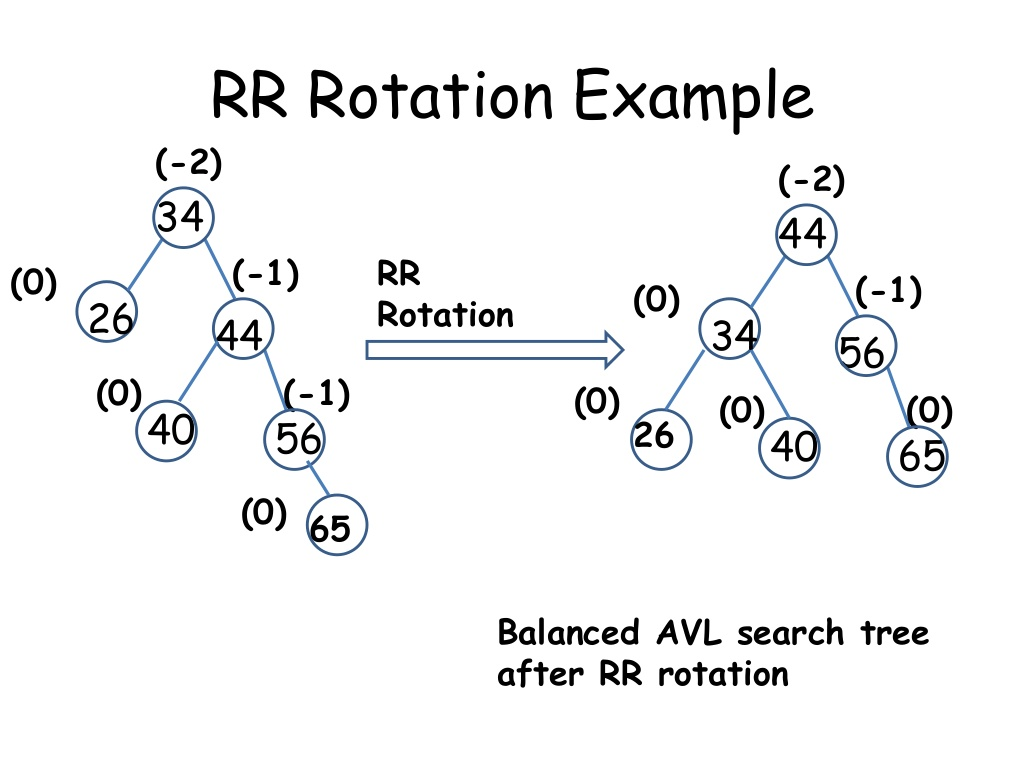
\includegraphics[width=300pt]{imagens/rr_rotation_example1.png}
  \label{fig_rr_rotation_example1}
\end{figure}
\end{frame}

%------------------------------------------------

\begin{frame}{Rotação RR}
% \scalebox{0.8}{
\begin{algorithm}[H]
\caption{RotaçãoRR} 
\label{RotacaoRR}
\Entrada{Ponteiro para o nodo desbalanceado $A$.}
\Inicio{
  B $\leftarrow$ A.dir \\
  A.dir $\leftarrow$ B.esq \\
  B.esq $\leftarrow$ A \\
  A.altura $\leftarrow$ maior(AlturaNodo(A.esq), AlturaNodo(A.dir)) + 1 \\
  B.altura $\leftarrow$ maior(AlturaNodo(B.dir), A.altura) + 1 \\
  A $\leftarrow$ B \\
}
\end{algorithm}
% }  
\tiny{Adaptado de \cite{Backes2016}}  
\end{frame}

%------------------------------------------------
\subsection{Rotação RL}
%------------------------------------------------

\begin{frame}{Rotação RL}
\begin{figure}[!h]
  \centering
   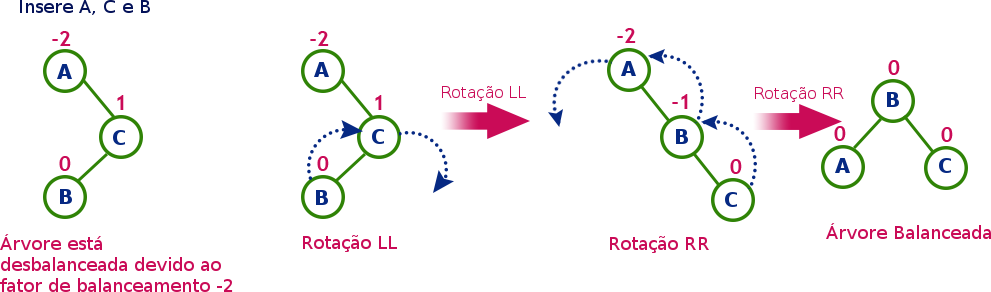
\includegraphics[width=300pt]{imagens/rotacao_rl.png}
  \label{fig_rotacao_rl}
\end{figure}
\end{frame}

%------------------------------------------------

\begin{frame}{Rotação RL}
\begin{figure}[!h]
  \centering
  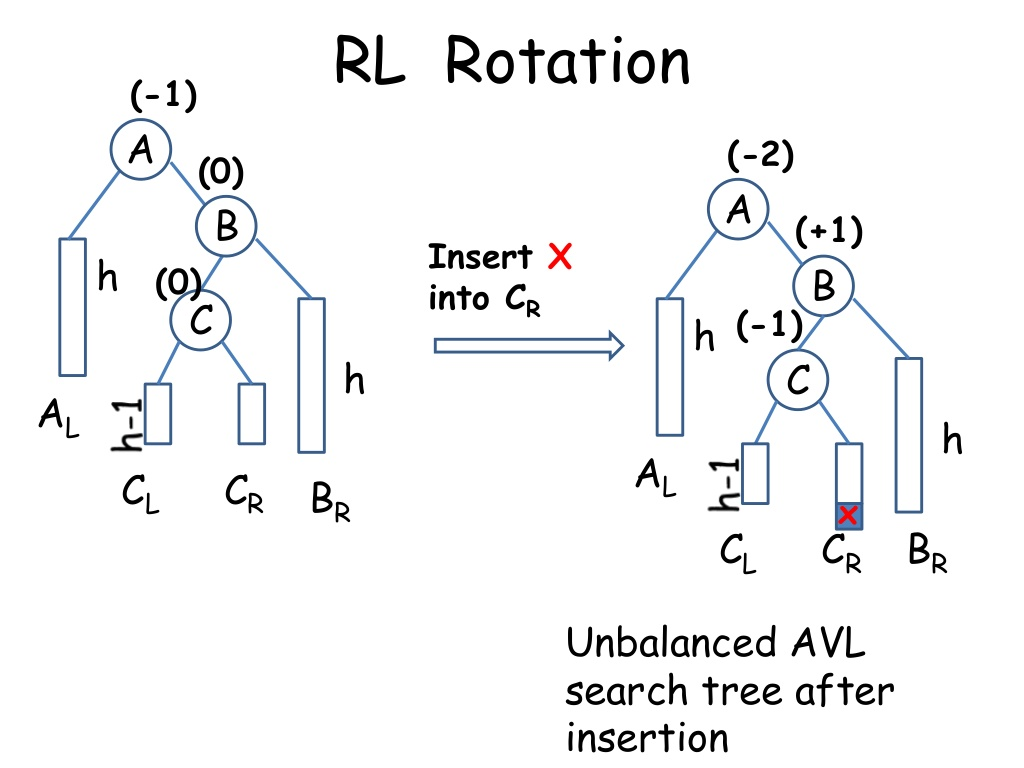
\includegraphics[width=300pt]{imagens/rl_rotation.png}
  \label{fig_rl_rotation}
\end{figure}
\end{frame}

%------------------------------------------------

\begin{frame}{Rotação RL}
\begin{figure}[!h]
  \centering
  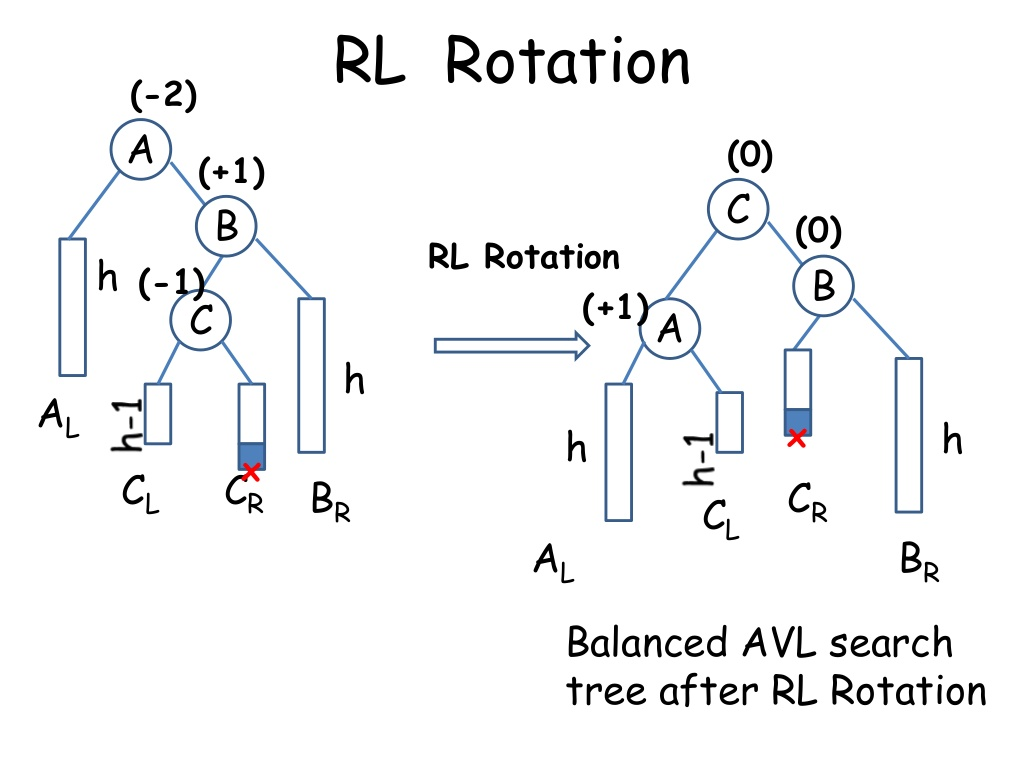
\includegraphics[width=300pt]{imagens/rl_rotation1.png}
  \label{fig_rl_rotation1}
\end{figure}
\end{frame}

%------------------------------------------------

\begin{frame}{Rotação RL}{Exemplo}
\begin{figure}[!h]
  \centering
  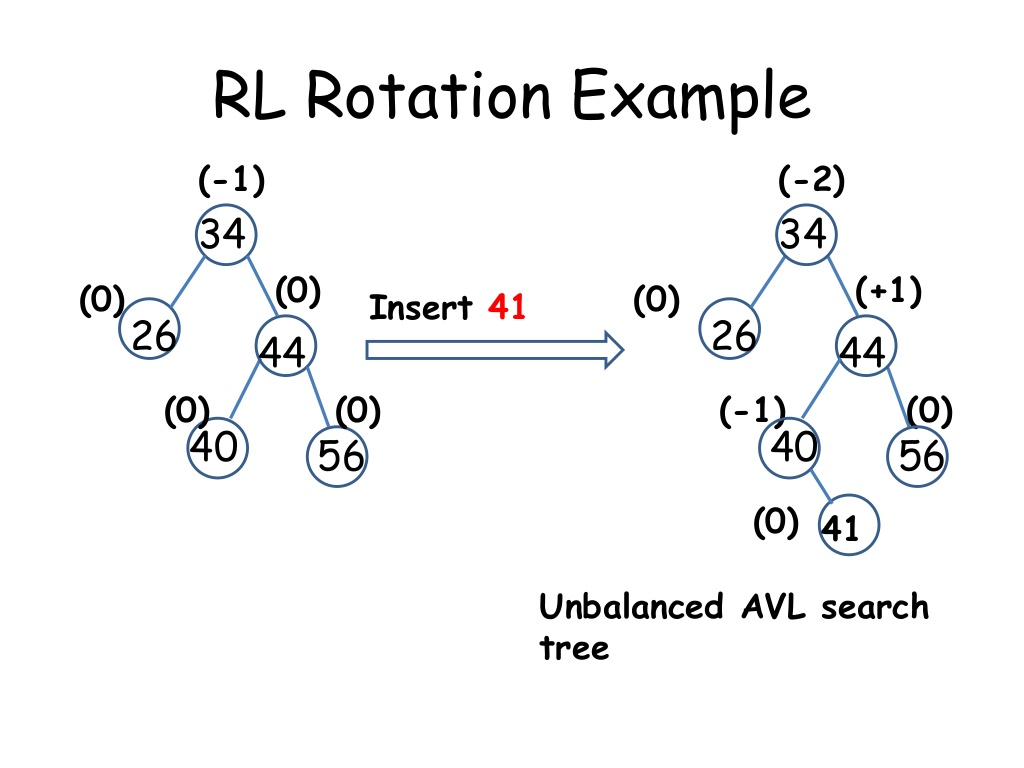
\includegraphics[width=300pt]{imagens/rl_rotation_example.png}
  \label{fig_rl_rotation_example}
\end{figure}
\end{frame}

%------------------------------------------------

\begin{frame}{Rotação RL}{Exemplo}
\begin{figure}[!h]
  \centering
  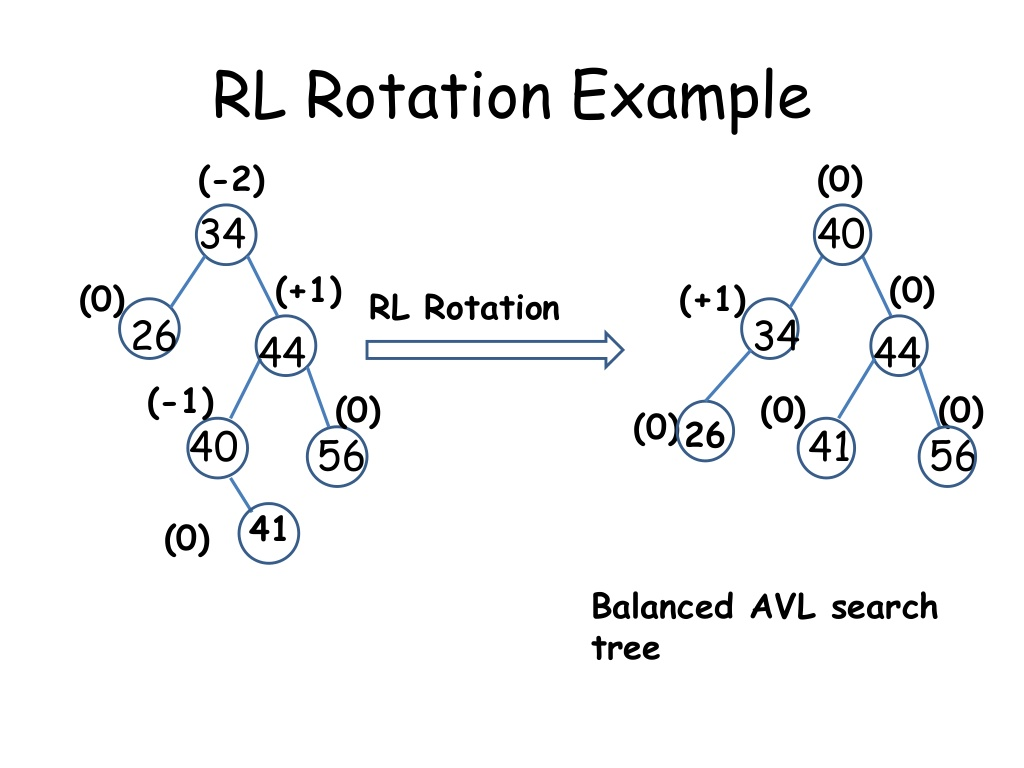
\includegraphics[width=300pt]{imagens/rl_rotation_example1.png}
  \label{fig_rl_rotation_example1}
\end{figure}
\end{frame}


%------------------------------------------------

\begin{frame}{Rotação RL}
% \scalebox{0.8}{
\begin{algorithm}[H]
\caption{RotaçãoRL} 
\label{RotacaoRL}
\Entrada{Ponteiro para a raiz $r$.}
\Inicio{
  RotaçãoLL(r.dir) \\
  RotaçãoRR(r) \\
}
\end{algorithm}
% }  
\tiny{Adaptado de \cite{Backes2016}}  
\end{frame}

%------------------------------------------------
\subsection{Rotação LR}
%------------------------------------------------

\begin{frame}{Rotação LR}
\begin{figure}[!h]
  \centering
   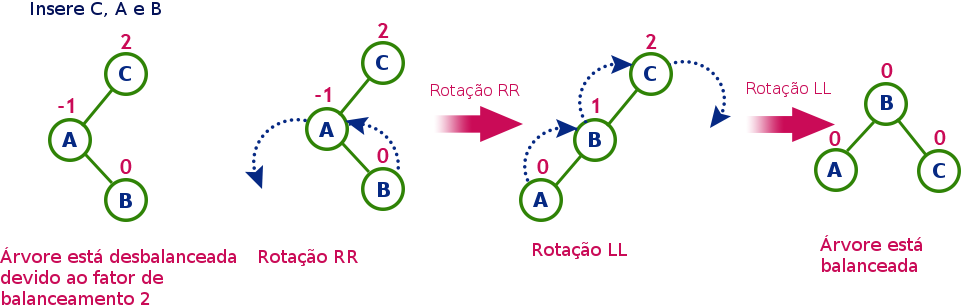
\includegraphics[width=300pt]{imagens/rotacao_lr.png}
  \label{fig_rotacao_lr}
\end{figure}
\end{frame}
%------------------------------------------------

\begin{frame}{Rotação RL}
\begin{figure}[!h]
  \centering
  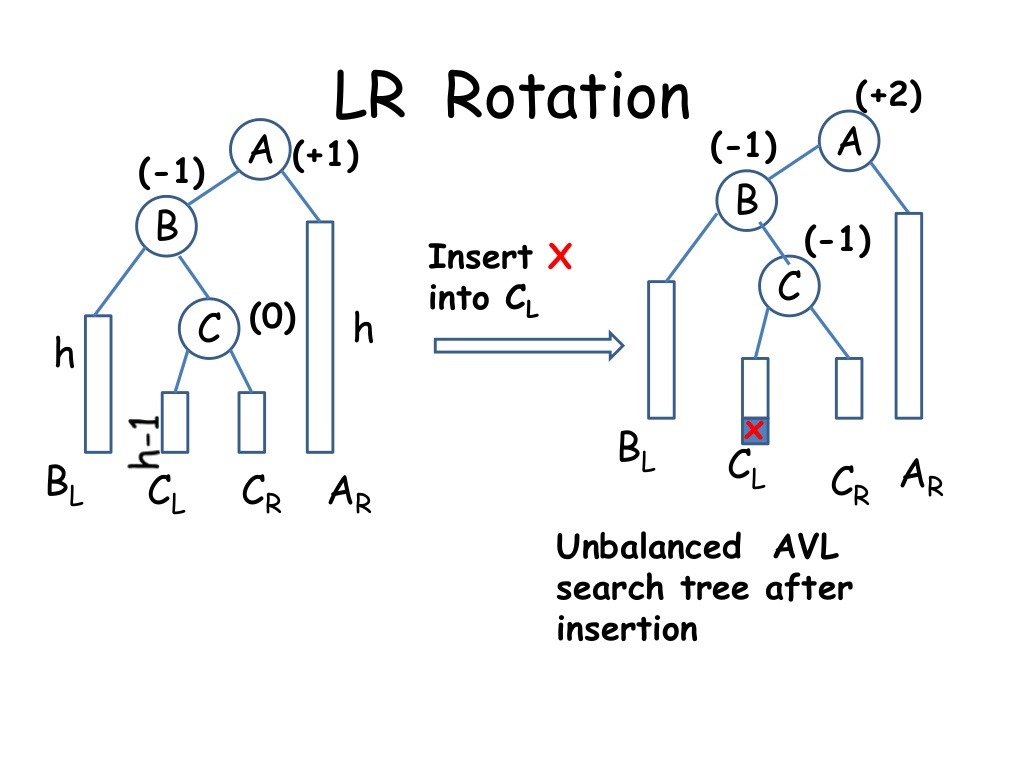
\includegraphics[width=300pt]{imagens/lr_rotation.png}
  \label{fig_lr_rotation}
\end{figure}
\end{frame}

%------------------------------------------------

\begin{frame}{Rotação RL}
\begin{figure}[!h]
  \centering
  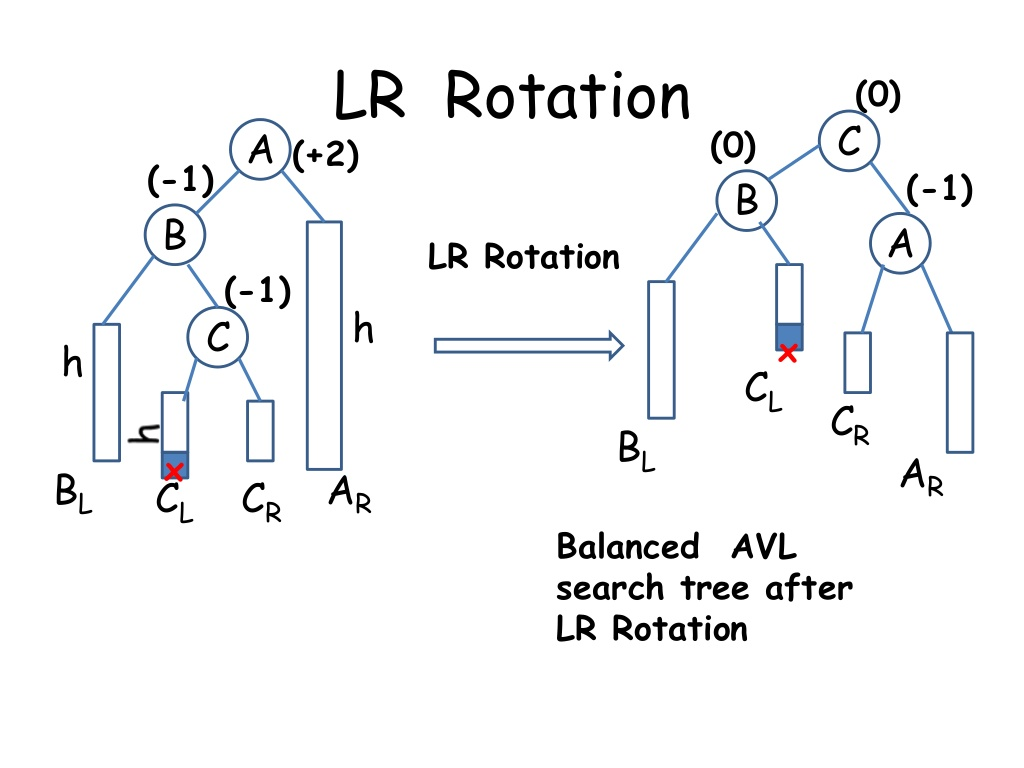
\includegraphics[width=300pt]{imagens/lr_rotation1.png}
  \label{fig_lr_rotation1}
\end{figure}
\end{frame}

%------------------------------------------------

\begin{frame}{Rotação RL}{Exemplo}
\begin{figure}[!h]
  \centering
  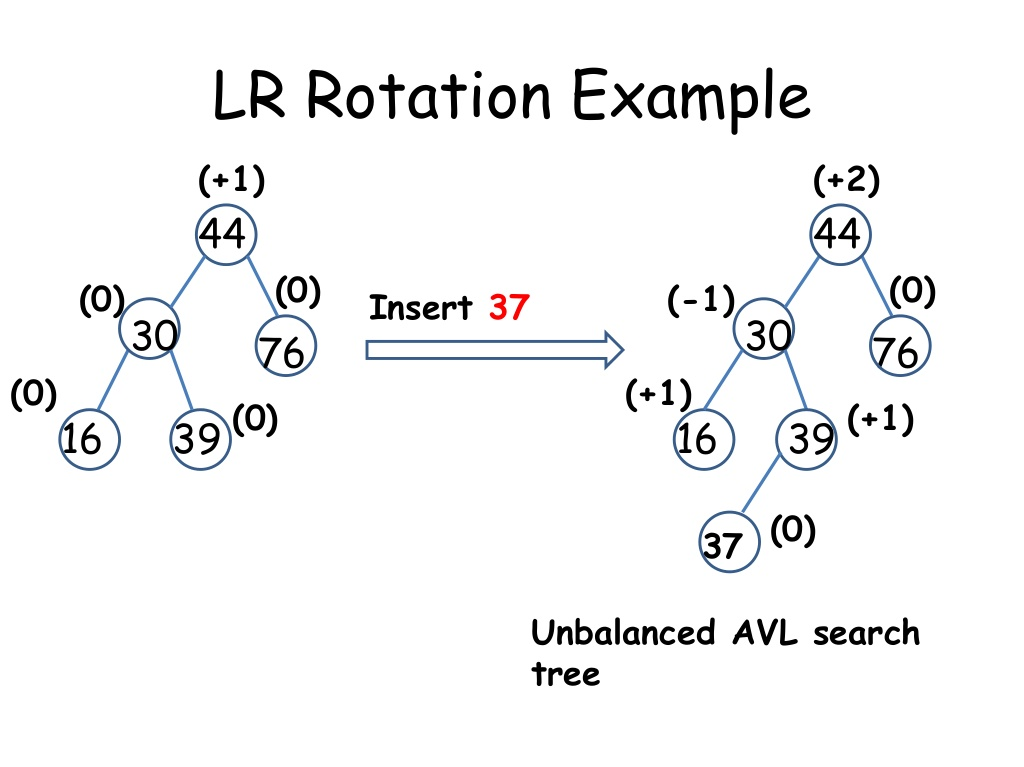
\includegraphics[width=300pt]{imagens/lr_rotation_example.png}
  \label{fig_lr_rotation_example}
\end{figure}
\end{frame}

%------------------------------------------------

\begin{frame}{Rotação RL}{Exemplo}
\begin{figure}[!h]
  \centering
  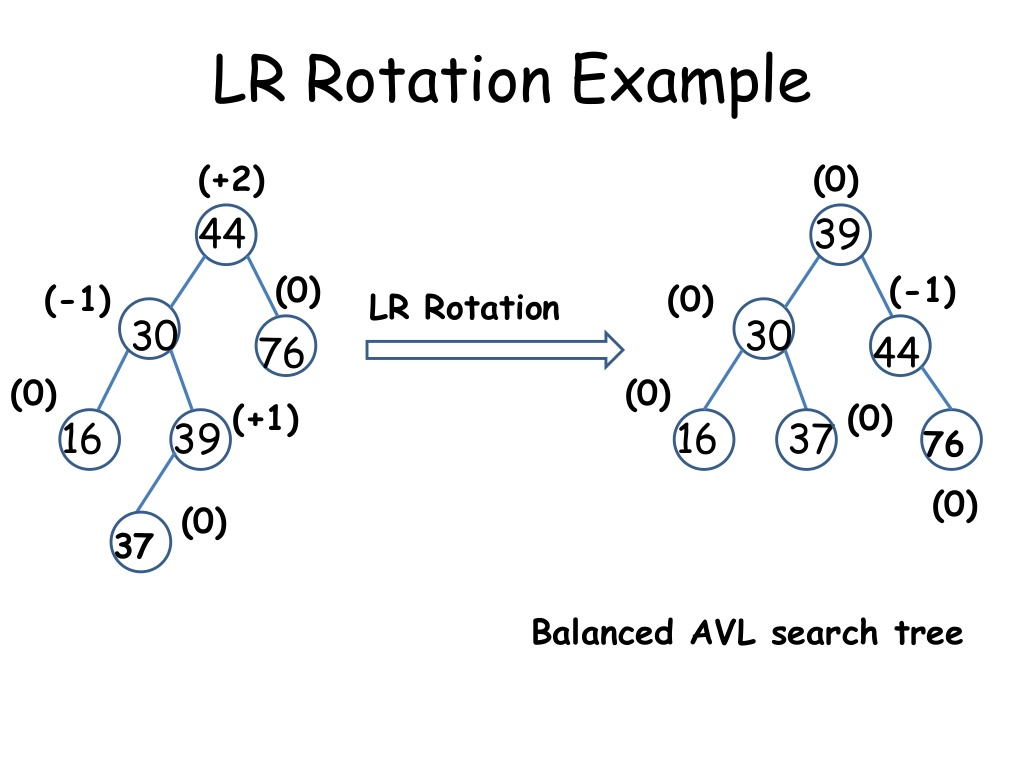
\includegraphics[width=300pt]{imagens/lr_rotation_example1.png}
  \label{fig_lr_rotation_example1}
\end{figure}
\end{frame}

%------------------------------------------------
\begin{frame}{Rotação LR}
% \scalebox{0.8}{
\begin{algorithm}[H]
\caption{RotaçãoLR} 
\label{RotacaoLR}
\Entrada{Ponteiro para a raiz $r$.}
\Inicio{
  RotaçãoRR(r.esq) \\
  RotaçãoLL(r) \\
}
\end{algorithm}
% }  
\tiny{Adaptado de \cite{Backes2016}}  
\end{frame}
%------------------------------------------------

% \begin{frame}{Introdução}{Rotações}
% \begin{itemize}
% \item As rotações são caracterizadas pelo ancestral mais próximo A do novo nó inserido $Y$ cujo fator de balanceamento passa a ser +2 ou -2.
% \begin{itemize}
% \item Rotação LL: $Y$ inserido na subárvore esquerda da subárvore esquerda de $A$.
% \item Rotação LR: $Y$ inserido na subárvore direita da subárvore esquerda de $A$.
% \item Rotação RR: $Y$ inserido na subárvore direita da subárvore direita de $A$.
% \item Rotação RL: $Y$ inserido na subárvore esquerda da subárvore direita de $A$.
% \end{itemize}
% \item Seja B o filho de $A$ no qual ocorreu a inserção de $Y$.
% \begin{itemize}
% \item Rotação LL ($A$ = +2; $B$ = +1)
% \item Rotação RR ($A$ = -2; $B$ = -1)
% \item Rotação LR ($A$ = +2; $B$ = -1)
% \item Rotação RL ($A$ = -2; $B$ = +1)
% \end{itemize}
% \item $C$ é o filho de $B$ no qual ocorreu a inserção de $Y$.
% \end{itemize}
% \end{frame}

%------------------------------------------------
\section{Inserção}
%------------------------------------------------


\begin{frame}{Inserção}
\begin{itemize}
 \item Para inserir um novo nodo em uma árvore AVL é necessário alocar espaço para o novo nodo e procurar a sua posição na árvore usando o seguinte conjunto de passos:
 \begin{enumerate}
  \item Primeiro, compare o {\bf valor} $x$ a ser inserido com a {\bf raiz}.
  \item Se $x$ for menor do que a {\bf raiz}: vá para a subárvore da {\bf esquerda}.
  \item Se $x$ for maior do que a {\bf raiz}: vá para a subárvore da {\bf direita}.
  \item Aplique o método recursivamente (pode ser feito sem recursão) até chegar a um {\bf nodo folha}.
 \end{enumerate}
 \item A inserção de num novo nodo em uma árvore AVL é exatamente igual à inserção na Árvore Binária de Busca (ABB). No entanto deve-se verificar o balanceamento e, caso necessário, realizar as rotações.
\end{itemize}
\end{frame}

%------------------------------------------------

\begin{frame}{Inserção}
\begin{itemize}
 \item O pseudocódigo a seguir trata o caso base do algoritmo recursivo: insere um novo nodo caso a árvore seja vazia:
\end{itemize}
\end{frame}

%------------------------------------------------

\begin{frame}{Inserção}{Pseudocódigo InserirAVL}
% \scalebox{0.5}{
\begin{algorithm}[H]
\caption{InserirAVL} 
\label{InserirAVL}
\Entrada{Ponteiro para a raiz $r$, item $x$.}
\Saida{V ou F}
\Inicio{
  \Se {( r = NULL)} {
    novo $\leftarrow$ ALOCA\_NODO() \\
    novo.item $\leftarrow$ x \\
    novo.altura $\leftarrow$ 0\\
    novo.esq $\leftarrow$ NULL \\
    novo.dir $\leftarrow$ NULL \\
    r $\leftarrow$ novo \\
    \Retorna Verdadeiro
   }
}
\rememberlines
\end{algorithm}
% }  
\end{frame}

%------------------------------------------------

\begin{frame}{Inserção}
\begin{itemize}
 \item O pseudocódigo a seguir, continuação do algoritmo anterior, trata os casos recursivos:
 \begin{enumerate}
  \item Verifica se $x$ é \underline{menor} que a {\bf raiz}: caso sim, insere recursivamente na subárvore da {\bf esquerda}.
  \item Caso seja \underline{maior}, insere recursivamente na subárvore da {\bf direita}.
  \item Se for \underline{igual}, significa que o valor já existe, e sua inserção termina retornando Falso.
 \end{enumerate}
 \item Esse conjunto de passos permite caminhar na árvore em busca do ponto de inserção do novo nodo. 
\end{itemize}
\end{frame}

%------------------------------------------------

\begin{frame}{Inserção}{Pseudocódigo InserirAVL}
\scalebox{0.5}{
\begin{algorithm}[H]
\resumenumbering
\caption{InserirAVL (continuação)} 
\label{InserirAVL2}
% \Entrada{Ponteiro para a raiz $r$, item $x$.}
% \Saida{V ou F}
\Inicio{
   atual $\leftarrow$ r \\
   \Se {(x $<$ atual.item)} {
     \Se {(InserirAVL(atual.esq, x))} { \label{inserir_avl_condicao1}
       \Se{(FatorBalanceamento(atual) $\geq 2$)} {
	  \Se {(x $<$ r.esq.item)} {
	    RotacaoLL(r) \\
	  }
	  \Senao {
	    RotacaoLR(r)\\
	  }
	}
      }
    }
    \Senao {
      \Se {(x $>$ atual.item)} {
	\Se{(InserirAVL(atual.dir, x))} { \label{inserir_avl_condicao2}
	  \Se{(FatorBalanceamento(atual) $\geq 2$)} {
	    \Se{(r.dir.item $<$ x)} {
	      RotacaoRR(r)\\
	    }
	    \Senao {
	      RotacaoRL(r)\\
	    }
	  }
	}
      }
      \Senao {
	\Retorna Falso
      }
    }
    atual.alt $\leftarrow$ maior(AlturaNodo(atual.esq),AlturaNodo(atual.dir)) + 1 \label{inserir_avl_atualiza_altura}\\
    \Retorna Verdadeiro    
}
\end{algorithm}
}  
\tiny{Adaptado de \cite{Backes2016}}  
\end{frame}

%------------------------------------------------

\begin{frame}{Inserção}
\begin{itemize}
 \item Após a inserção, é realizado o rebalanceamento da árvore:
 \begin{enumerate}
  \item Se a inserção foi feita na subárvore da {\bf esquerda} do nodo {\bf atual}, devemos esconter entre a {\bf rotação LL} e a {\bf rotação LR} (linha \ref{inserir_avl_condicao1}).
  \begin{itemize}
  \item Se $x$ for \underline{menor} do que o valor do filho à {\bf esquerda} de {\bf atual}, isso significa que o valor foi inserido na subárvore esquerda do filho à esquerda de {\bf atual}: necessária uma {\bf rotação LL}.
  \item Caso contrário, é necessária uma {\bf rotação LR}.
  \end{itemize}
  \item Se a inserção foi feita na subárvore da {\bf direita} do nodo {\bf atual}, devemos esconter entre a {\bf rotação RR} e a {\bf rotação RL} (linha \ref{inserir_avl_condicao2}).
  \begin{itemize}
  \item Se $x$ for \underline{maior} do que o valor do filho à {\bf direita} de {\bf atual}, isso significa que o valor foi inserido na subárvore direita do filho à direita de {\bf atual}: necessária uma {\bf rotação RR}.
  \item Caso contrário, é necessária uma {\bf rotação RL}.
  \end{itemize}  
 \end{enumerate}
\item Por fim, atualiza a altura do nodo {\bf atual} (linha \ref{inserir_avl_atualiza_altura}).
\end{itemize}
\end{frame}

%------------------------------------------------

\subsection{Exemplo}

\begin{frame}{Inserção}{Exemplo}
Construa uma árvore AVL de busca inserindo os seguintes elementos na ordem de sua ocorrência: 64, 1, 14, 26, 13, 110, 98, 85.
\end{frame}

%------------------------------------------------

\begin{frame}{Inserção}{Exemplo}
\begin{figure}[!h]
  \centering
  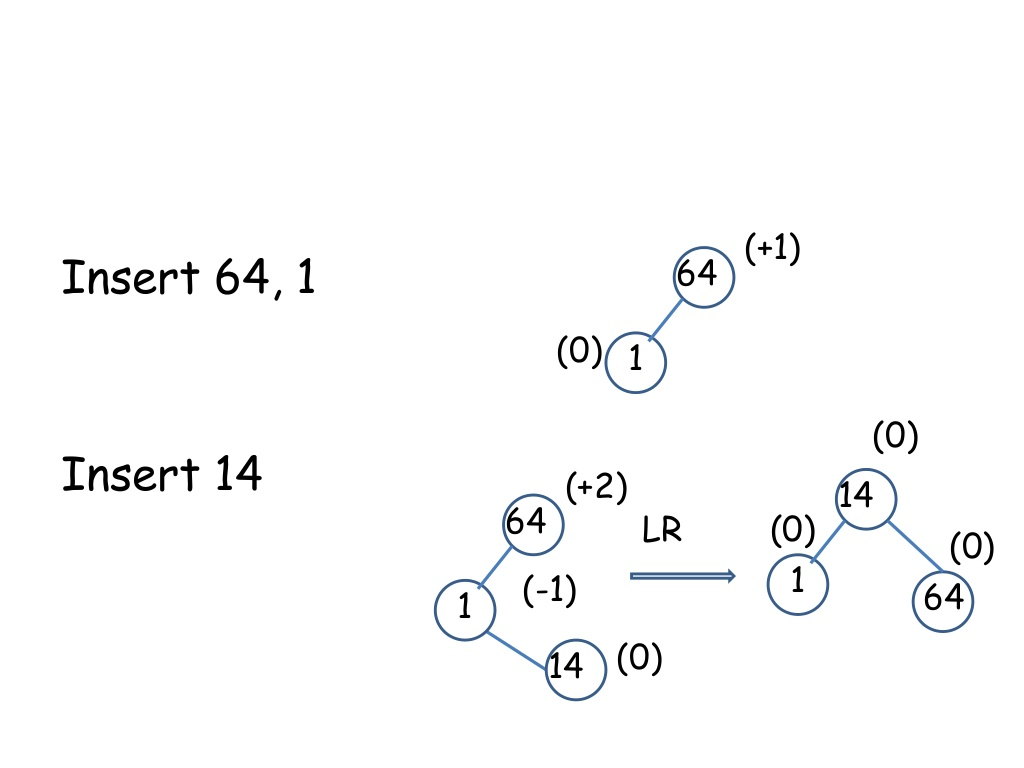
\includegraphics[width=250pt]{imagens/exemplo_insercao1.png}
  \label{fig_exemplo_insercao1}
\end{figure}
\end{frame}


%------------------------------------------------

\begin{frame}{Inserção}{Exemplo}
\begin{figure}[!h]
  \centering
  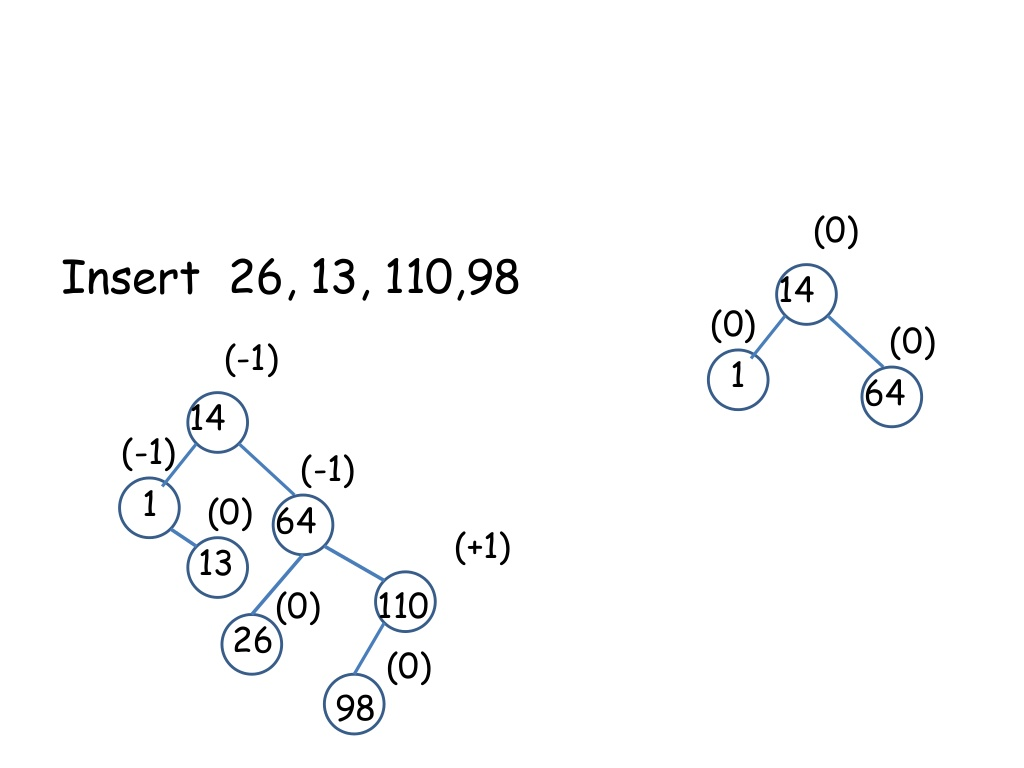
\includegraphics[width=250pt]{imagens/exemplo_insercao2.png}
  \label{fig_exemplo_insercao2}
\end{figure}
\end{frame}


%------------------------------------------------

\begin{frame}{Inserção}{Exemplo}
\begin{figure}[!h]
  \centering
  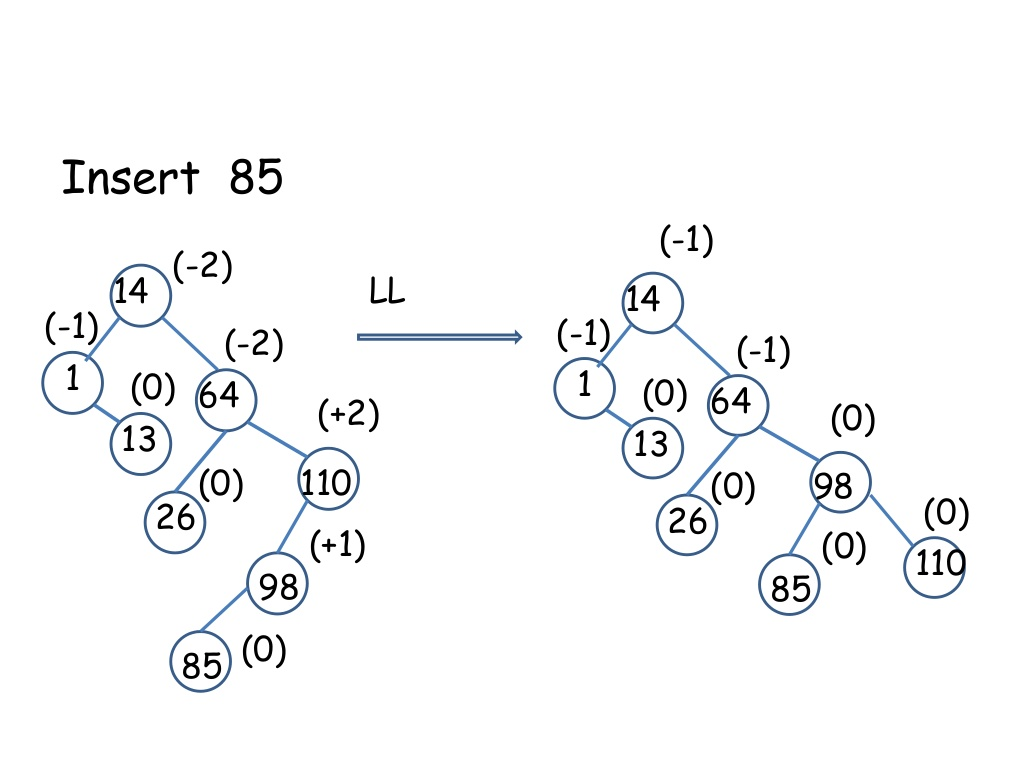
\includegraphics[width=300pt]{imagens/exemplo_insercao3.png}
  \label{fig_exemplo_insercao3}
\end{figure}
\end{frame}

%------------------------------------------------
% 
% \begin{frame}{Inserção}{Pseudocódigo CriaNodo}
% % \scalebox{0.8}{
% \begin{algorithm}[H]
% \caption{CriaNodo} 
% \label{CriaNodo}
% \Entrada{Item $x$ a ser armazenado no nodo.}
% \Saida{Ponteiro para o novo nodo.}
% \Inicio{
%     n $\leftarrow$ ALOCA\_NODO() \\
%     n.item $\leftarrow$ x \\
%     n.altura $\leftarrow$ 0\\
%     n.esq $\leftarrow$ NULL \\
%     n.dir $\leftarrow$ NULL \\
%     \Retorna n
% }
% \end{algorithm}
% % }  
% \end{frame}

%------------------------------------------------
% 
% \begin{frame}{Inserção}{Pseudocódigo InserirAVL}
% \scalebox{0.5}{
% \begin{algorithm}[H]
% \caption{InserirAVL} 
% \label{InserirAVL}
% \Entrada{Ponteiro para a raiz $r$, item $x$.}
% \Saida{V ou F}
% \Inicio{
%   \Se {( r = NULL)} {
%     novo $\leftarrow$ CriaNodo(x) \\
%     r $\leftarrow$ novo \\
%     \Retorna Verdadeiro
%    }
%    atual $\leftarrow$ r \\
%    \Se {(x $<$ atual.item)} {
%      \Se {(InserirAVL(atual.esq, x))} {
%        \Se{(FatorBalanceamento(atual) $\geq 2$)} {
% 	  \Se {(x $<$ r.esq.item)} {
% 	    RotacaoLL(r) \\
% 	  }
% 	  \Senao {
% 	    RotacaoRR(r)\\
% 	  }
% 	}
%       }
%     }
%     \Senao {
%       \Se {(x $>$ atual.item)} {
% 	\Se{(InserirAVL(atual.dir, x))} {
% 	  \Se{(FatorBalanceamento(atual) $\geq 2$)} {
% 	    \Se{(r.dir.item $<$ x)} {
% 	      RotacaoRR(r)\\
% 	    }
% 	    \Senao {
% 	      RotacaoLL(r)\\
% 	    }
% 	  }
% 	}
%       }
%       \Senao {
% 	\Retorna Falso
%       }
%     }
%     atual.alt $\leftarrow$ maior(AlturaNodo(atual.esq),AlturaNodo(atual.dir)) + 1\\
%     \Retorna Verdadeiro
% }
% \end{algorithm}
% }  
% \end{frame}

%------------------------------------------------
\section{Remoção}
%------------------------------------------------

\begin{frame}{Remoção}
Para remover um nodo recursivamente em uma árvore AVL é necessário o seguinte conjunto de passos:
 \begin{itemize}
  \item Primeiro, compare o {\bf valor} $x$ a ser removido com a {\bf raiz}.
  \begin{itemize}
  \item Se $x$ for menor do que a {\bf raiz}, remova recursivamente na subárvore da {\bf esquerda}.
  \item Se $x$ for maior do que a {\bf raiz}, remova recursivamente na subárvore da {\bf direita}.
  \end{itemize}
  \item As chamadas recursivas param em duas situações:
  \begin{enumerate}
  \item Encontra-se o nodo que possui valor $x$.
  \item Ou quando a raiz da subárvore é igual a NULL (indicando que o valor não existe na árvore).
  \end{enumerate}
 \end{itemize}
A remoção de num nodo em uma árvore AVL é exatamente igual à remoção na ABB. Também pode ser feita de forma iterativa. No entanto deve-se verificar o balanceamento e, caso necessário, realizar as rotações. 
\end{frame}


\begin{frame}{Remoção}
\begin{itemize}
 \item Para balancear a árvore após a remoção de um nodo, valem as mesmas regras da inserção.
 \item No entanto, há uma diferença: remover um nodo da subárvore da direita equivale a inserir um nodo na subárvore da esquerda.
 \item A seguir, um exemplo que ilustra um caso em que a remoção em uma árvore AVL produz exatemente o mesmo tipo de rotação que a inserção em outra árvore.
\end{itemize}
\end{frame}

%------------------------------------------------

\begin{frame}{Remoção}{Exemplo}

\begin{figure}[!h]
  \centering
  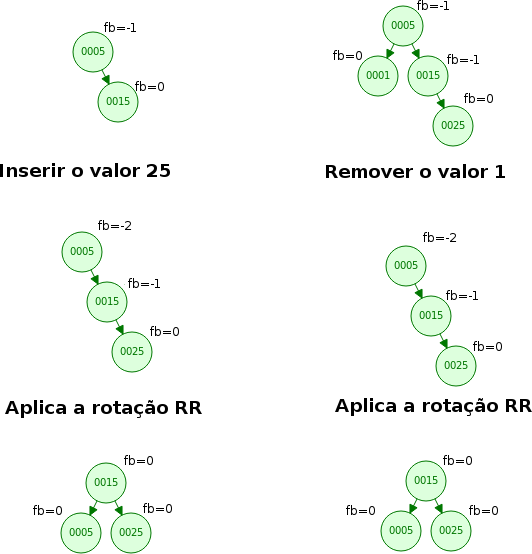
\includegraphics[width=180pt]{imagens/exemplo_remocao.png}
  \label{fig_exemplo_remocao}
\end{figure}
\end{frame}

%------------------------------------------------

\begin{frame}{Remoção}{Algoritmo ProcuraMaior}
\begin{itemize}
 \item A fim de remover um nodo, o algoritmo fará uso de uma outra função: {\bf ProcuraMaior()}, cuja implementação é mostrada a seguir. 
 \item Essa função é usada para procurar o {\bf nodo mais à direita} a partir de certo nodo da árvore, {\bf atual}.
 \item Será utilizada para encontrar o nodo {\bf antecessor} ao nodo que será removido da árvore.
 \begin{itemize}
 \item O nodo antecessor é o nodo mais à direita da subárvore da esquerda.
 \end{itemize} 
\end{itemize}
\end{frame}

%------------------------------------------------

\begin{frame}{Remoção}{Algoritmo ProcuraMaior}
% \scalebox{0.8}{
\begin{algorithm}[H]
\caption{ProcuraMaior} 
\label{ProcuraMaior}
\Entrada{Ponteiro para o nodo {\bf atual}.}
\Saida{Ponteiro para o maior valor a partir do nodo {\bf atual}.}
\Inicio{
    n1 $\leftarrow$ atual\\
    n2 $\leftarrow$ atual.dir\\
    \Enqto {(n2$\neq$ NULL)} {
      n1 $\leftarrow$ n2\\
      n2 $\leftarrow$ n2.dir\\
    }
    \Retorna n1
}
\end{algorithm}
% }  
\tiny{Adaptado de \cite{Backes2016}}  
\end{frame}

%------------------------------------------------

\begin{frame}{Remoção}{Algoritmo RemoverAVL}
Para realizar a remoção de um elemento da árvore, realiza-se os seguintes passos:
\begin{itemize}
 \item Primeiramente, a função verifica se o conteúdo do ponteiro é igual a NULL. A condição é verdadeira em dois casos:
 \begin{itemize}
 \item A árvore é vazia.
 \item Ao descer, recursivamente, na árvore, o nodo de onde viemos era um nodo folha.
 \end{itemize}
 \item Seja qual for o caso, retorna Falso para indicar que o valor não se encontra na árvore.
\end{itemize}
\end{frame}

%------------------------------------------------

\begin{frame}{Remoção}{Algoritmo RemoverAVL}
 Em seguida, consideramos três casos ao remover $x$:
 \begin{enumerate}
 \item Se  $(x < raiz.item)$:
 \begin{itemize}
 \item Deve-se, recursivamente, remover $x$ na subárvore à {\bf esquerda} da {\bf raiz}.
\end{itemize}  
 \item Se $(x > raiz.item)$:
 \begin{itemize}
 \item Deve-se, recursivamente, remover $x$ da subárvore à {\bf direita} da {\bf raiz}. 
\end{itemize}  
 \item Caso contrário, $x$ é igual ao valor do nodo raiz:
 \begin{itemize}
 \item Encontrou o nodo a ser removido.
\end{itemize} 
\end{enumerate}
A seguir, tem-se o pseudocódigo referente a remoção em uma árvore AVL.
\end{frame}

%------------------------------------------------

\begin{frame}{Remoção}{Algoritmo RemoverAVL}
\scalebox{0.55}{
\begin{algorithm}[H]
\caption{RemoverAVL} 
\label{RemoverAVL}
\Entrada{Ponteiro para a raiz $r$, item $x$.}
\Saida{V ou F}
\Inicio{
  \Se{(r = NULL)} { \label{remover_avl_arvore_vazia}
    \Retorna Falso
  }
  \Se{(x $<$ r.item)} { \label{remover_avl_x_menor}
    \Se{(RemoverAVL(r.esq, x))} { \label{remover_avl_teste_recursivo1}
      \Se{(FatorBalanceamento(r) $\geq$ 2)} { \label{remover_avl_teste_balanceamento_inicio1}
			\Se {(AlturaNodo(r.dir.esq) $\leq$ AlturaNodo(r.dir.dir))} {
	  			RotacaoRR(r) \\
			}
			\Senao {
	  			RotacaoRL(r) \\
			}
      } \label{remover_avl_teste_balanceamento_fim1}
    }
  }
  \Se{(x $>$ r.item )} {  \label{remover_avl_x_maior}
    \Se{(RemoverAVL(r.dir, x))} { \label{remover_avl_teste_recursivo2}
      \Se{(FatorBalanceamento(r) $\geq$ 2)} { \label{remover_avl_teste_balanceamento_inicio2}
			\Se {(AlturaNodo(r.esq.dir) $\leq$ AlturaNodo(r.esq.esq))} {
				  RotacaoLL(r) \\
			}
			\Senao {
				  RotacaoLR(r) \\
			}
      	} \label{remover_avl_teste_balanceamento_fim2}	
    } 
  }  
  \rememberlines
}
\end{algorithm}
}\tiny{Adaptado de \cite{Backes2016}}  
\end{frame}

%------------------------------------------------

\begin{frame}{Remoção}{Algoritmo RemoverAVL}
\begin{itemize}
\item Primeiramente, verifica se a árvore está vazia (linha \ref{remover_avl_arvore_vazia}).
\begin{itemize}
\item Em caso positivo, retorna falso, pois não foi possível remover o elemento.
\end{itemize} 
\item Caso contrário, verifica se $x < raiz.item$ (linha \ref{remover_avl_x_menor}).
\begin{itemize}
\item Caso sim, remove recursivamente o nodo, passando a subárvore da esquerda como nodo {\bf raiz} (linha \ref{remover_avl_teste_recursivo1}).
\item Em seguida, realiza o balanceamento (linhas \ref{remover_avl_teste_balanceamento_inicio1}-\ref{remover_avl_teste_balanceamento_fim1}). O balanceamento segue a mesma ideia da inserção.
\end{itemize}
\item Em seguida, verifica se $x > raiz.item$ (linha \ref{remover_avl_x_maior}).
\begin{itemize}
\item Caso sim, remove recursivamente o nodo (linha \ref{remover_avl_teste_recursivo2}).
\item Em seguida, realiza o balanceamento (linhas \ref{remover_avl_teste_balanceamento_inicio2}-\ref{remover_avl_teste_balanceamento_fim2}).
\end{itemize}
\item A seguir, apresenta-se a continuação do algoritmo.
\end{itemize}
\end{frame}


%------------------------------------------------

\begin{frame}{Remoção}{Algoritmo RemoverAVL}
\scalebox{0.5}{
\begin{algorithm}[H]
\caption{RemoverAVL (Continuação)} 
\label{RemoverAVL2}
\resumenumbering
\Inicio{
  \Se {(r.item = x)} { \label{remover_avl_remocao_inicio}
    \Se{(r.esq = NULL) ou (r.dir = NULL)} { \label{remover_avl_nodo_folha}
      removerNodo $\leftarrow$ r \label{remover_avl_nodo_auxiliar} \\ 
      \Se {(r.esq $\neq$ NULL)} { \label{remover_avl_nodo_folha_atualiza_filho_inicio}
			r $\leftarrow$ r.esq \\
      }
      \Senao { \label{remover_avl_nodo_folha_raiz_null_inicio}
			r $\leftarrow$ r.dir \label{remover_avl_nodo_folha_atualiza_raiz_null_fim}\\
      } \label{remover_avl_nodo_folha_atualiza_filho_fim}
      DESALOCA\_NODO(removerNodo) \label{remover_avl_nodo_folha_libera_memoria} \\      
    } 
    \Senao { \label{remover_avl_nodo_dois_filhos_inicio}
      	antecessor $\leftarrow$ ProcuraMaior(r.dir) \label{remover_avl_busca_antecessor} \\
      	r.item $\leftrightarrow$ antecessor.item \CommentSty{// Troca os valores.} \label{remover_avl_troca_raiz_antecessor} \\
      	RemoverAVL(r.dir, antecessor.item) \label{remover_avl_remover_antecessor} \\
      	\Se {(FatorBalanceamento(r) $\geq$ 2)} { \label{remover_avl_verifica_balanceamento}
			\Se{AlturaNodo(r.esq.dir) $\leq$ AlturaNodo(r.esq.esq)} { \label{remover_avl_verifica_altura}
	  			RotaçãoLL(r) \label{remover_avl_rotacao_simples} \\
		}
		\Senao {
	  		RotaçãoLR(r) \label{remover_avl_rotacao_dupla} \\
		}
      }
      \Se{(r $\neq$ NULL)} {
			r.altura $\leftarrow$ maior(AlturaNodo(r.esq), AlturaNodo(r.dir)) + 1 \\
      }
      \Retorna Verdadeiro
    } \label{remover_avl_nodo_dois_filhos_fim}
    r.altura $\leftarrow$ maior(AlturaNodo(r.esq), AlturaNodo(r.dir)) + 1 \\
    \Retorna Verdadeiro \label{remover_avl_retorna_verdadeiro}
  }
}  \label{remover_avl_remocao_fim}
\end{algorithm}
}\tiny{Adaptado de \cite{Backes2016}}  
\end{frame}


%------------------------------------------------

\begin{frame}{Remoção}{Algoritmo RemoverAVL}
\begin{itemize}
\item O caso base da remoção é tratado nas linhas  \ref{remover_avl_remocao_inicio}-\ref{remover_avl_remocao_fim}.
\item Inicialmente, verifica se o nodo atual ({\bf raiz}) é um nodo folha (sem filhos) ou se ele possui apenas um dos filhos (linha \ref{remover_avl_nodo_folha}).
\begin{itemize}
\item Caso seja verdade, copia a raiz para um nodo auxiliar ({\bf removerNodo} - linha \ref{remover_avl_nodo_auxiliar}) e um dos filhos assume o lugar do pai (linhas \ref{remover_avl_nodo_folha_atualiza_filho_inicio}-\ref{remover_avl_nodo_folha_atualiza_filho_fim}). Se for nodo folha, a raiz recebe NULL (linhas \ref{remover_avl_nodo_folha_raiz_null_inicio}, \ref{remover_avl_nodo_folha_atualiza_raiz_null_fim}).
\begin{itemize}
\item Em seguida, libera a memória ocupada pelo nodo (linha \ref{remover_avl_nodo_folha_libera_memoria}).
\end{itemize}
\item Caso contrário, significa que o nó {\bf raiz} possui dois filhos. 
\begin{itemize}
\item Nesse caso, utiliza-se a função {\bf ProcuraMaior()} para encontrar o antecessor da {\bf raiz} (nodo mais à direita da subárvore da esquerda) - linha \ref{remover_avl_busca_antecessor}.
\item Em seguida, troca os valores entre o nodo {\bf raiz} e seu {\bf antecessor} (linha \ref{remover_avl_troca_raiz_antecessor}).
\item Chama novamente a função {\bf RemoverAVL()}, desta vez para remover o nodo antecessor {\bf ProcuraMaior()} (linha \ref{remover_avl_remover_antecessor}).
\item Por fim, trata o balanceamento (linha \ref{remover_avl_verifica_balanceamento}), o qual poderá ser uma {\bf rotação LL}, se a altura da árvore direita do filho esquerdo for menor ou igual a da árvore esquerda do filho esquerdo (linhas \ref{remover_avl_verifica_altura}, \ref{remover_avl_rotacao_simples}), ou uma {\bf rotação LR}, no caso contrário (linha \ref{remover_avl_rotacao_dupla}).
\end{itemize}
\end{itemize}
\end{itemize}
\end{frame}

%------------------------------------------------

\begin{frame}{Remoção}{Algoritmo RemoverAVL}
\begin{itemize}
\item Terminado o processo de remoção, atualiza a altura do nodo e retorna {\bf verdadeiro} (linha \ref{remover_avl_retorna_verdadeiro}), indicando que o elemento foi removido com sucesso.
\end{itemize}
\end{frame}

%------------------------------------------------
\subsection{Exemplo}
%------------------------------------------------

\begin{frame}{Remoção}{Exemplo}
\begin{figure}[!h]
  \centering
  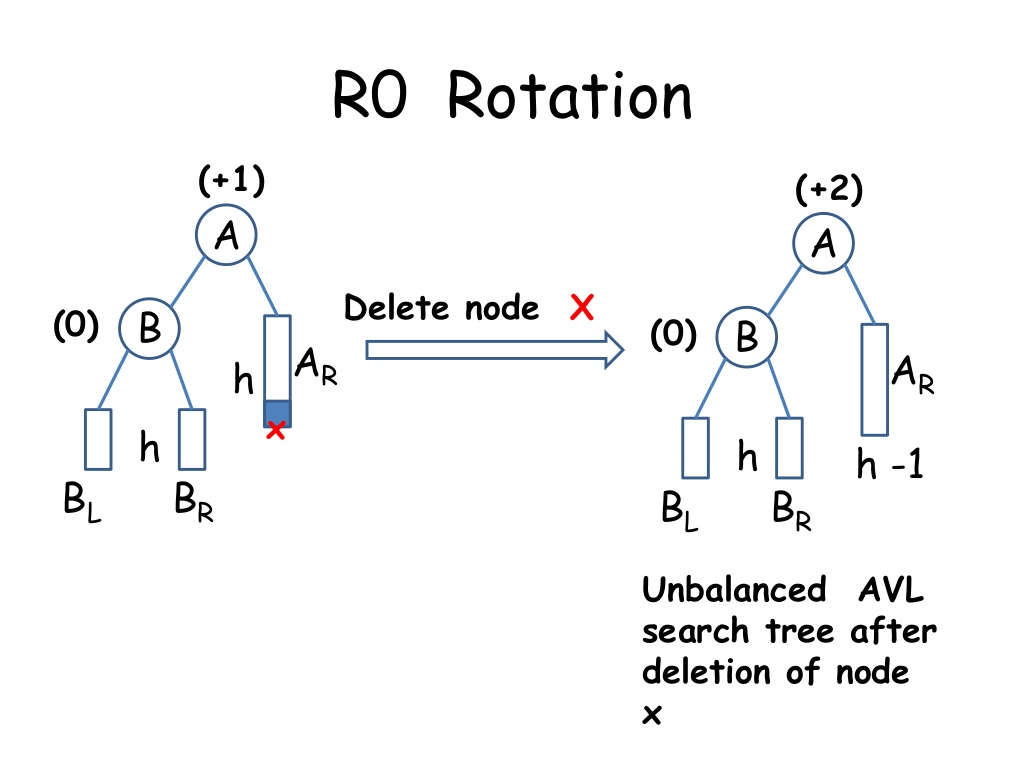
\includegraphics[width=250pt]{imagens/exemplo_remocao1.png}
  \label{fig_exemplo_remocao1}
\end{figure}
\end{frame}


%------------------------------------------------

\begin{frame}{Remoção}{Exemplo}
\begin{figure}[!h]
  \centering
  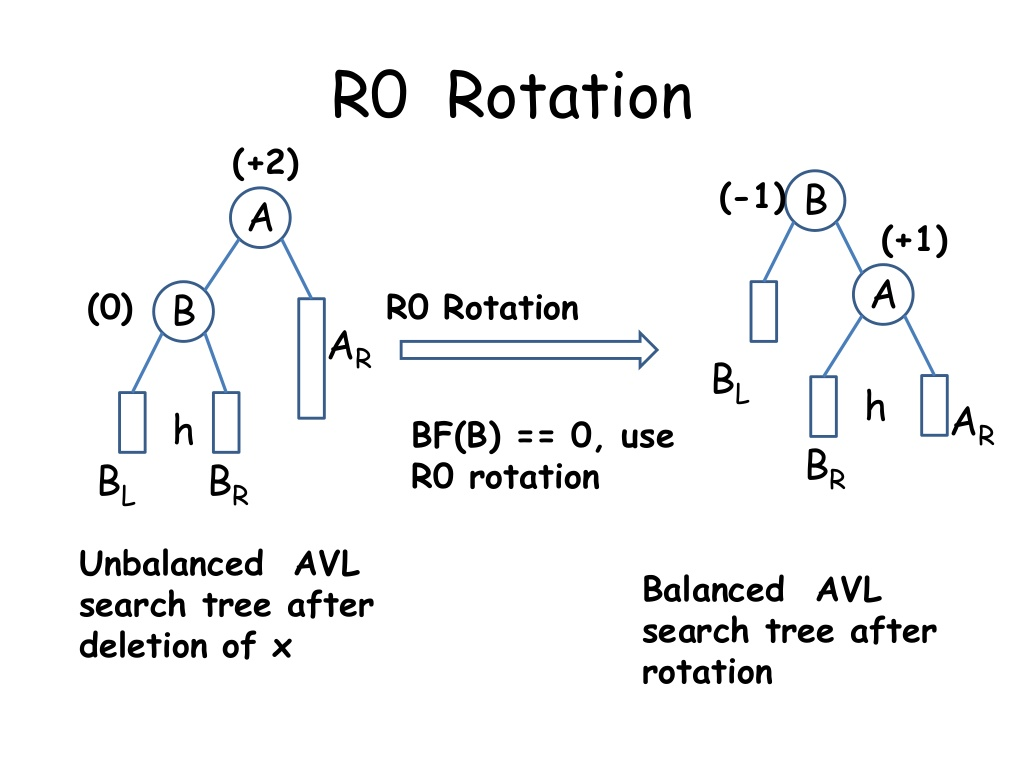
\includegraphics[width=250pt]{imagens/exemplo_remocao2.png}
  \label{fig_exemplo_remocao2}
\end{figure}
\end{frame}


%------------------------------------------------

\begin{frame}{Remoção}{Exemplo}
\begin{figure}[!h]
  \centering
  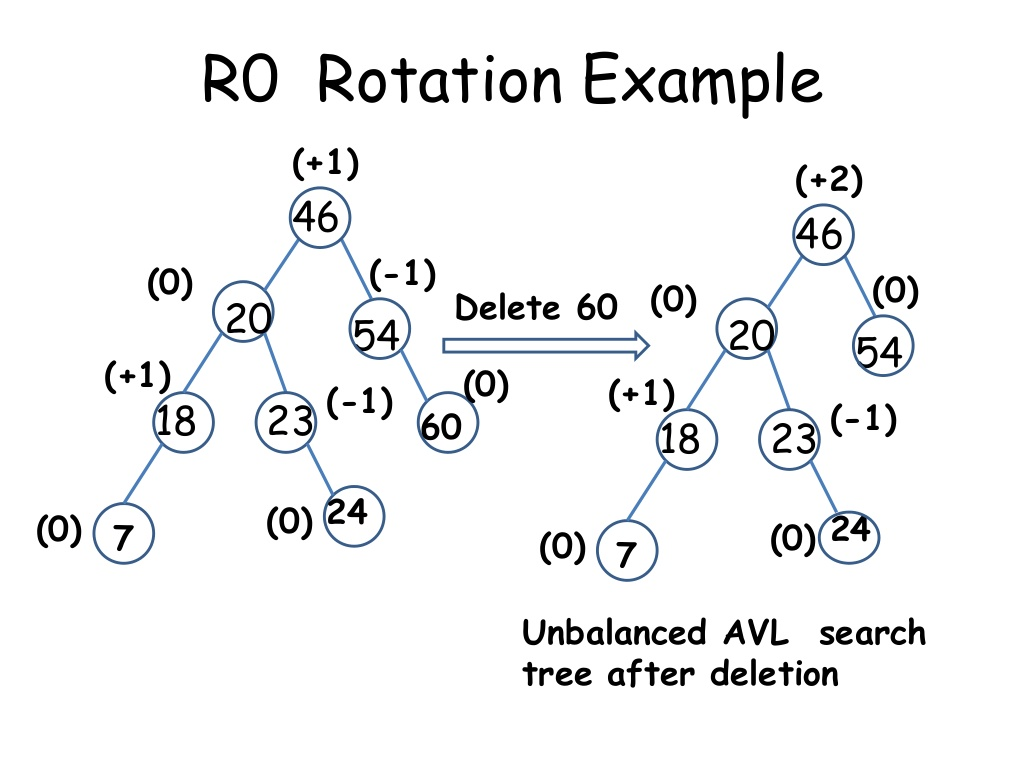
\includegraphics[width=250pt]{imagens/exemplo_remocao3.png}
  \label{fig_exemplo_remocao3}
\end{figure}
\end{frame}


%------------------------------------------------

\begin{frame}{Remoção}{Exemplo}
\begin{figure}[!h]
  \centering
  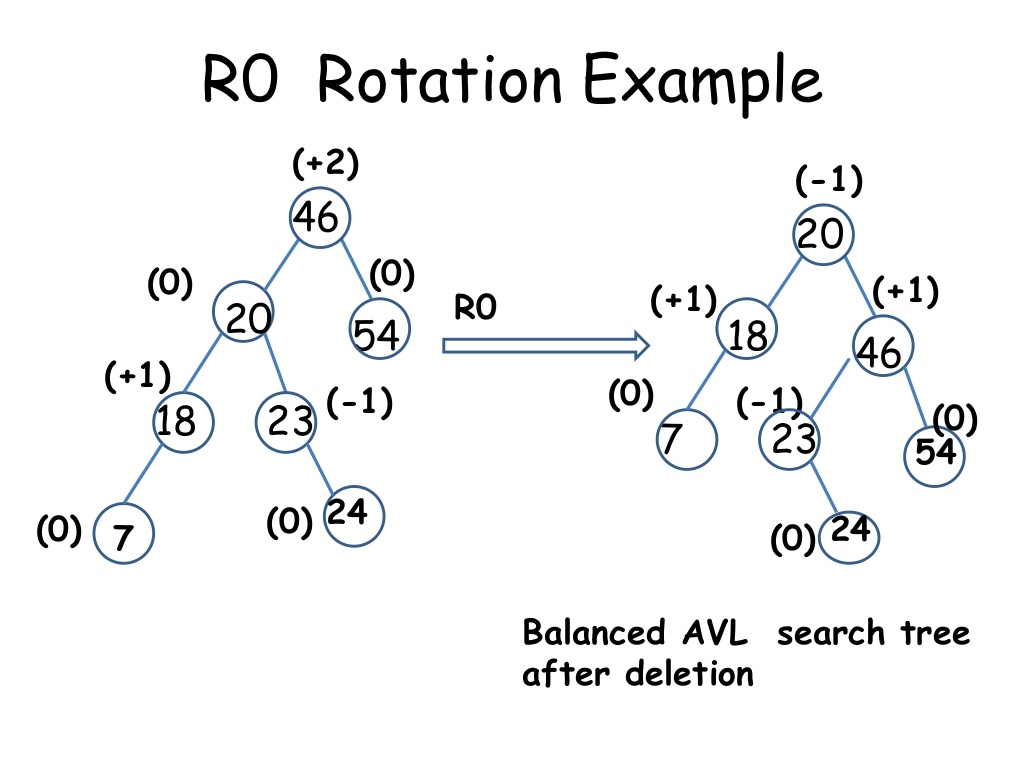
\includegraphics[width=250pt]{imagens/exemplo_remocao4.png}
  \label{fig_exemplo_remocao4}
\end{figure}
\end{frame}


%------------------------------------------------

\begin{frame}{Remoção}{Exemplo}
\begin{figure}[!h]
  \centering
  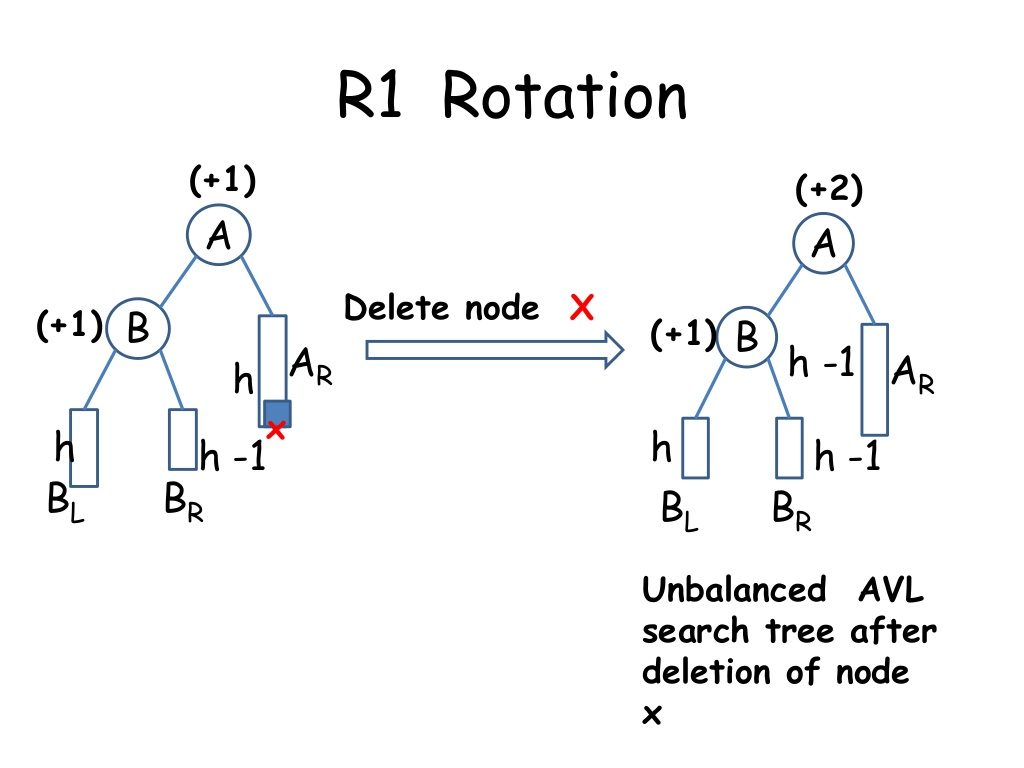
\includegraphics[width=250pt]{imagens/exemplo_remocao5.png}
  \label{fig_exemplo_remocao5}
\end{figure}
\end{frame}

%------------------------------------------------

\begin{frame}{Remoção}{Exemplo}
\begin{figure}[!h]
  \centering
  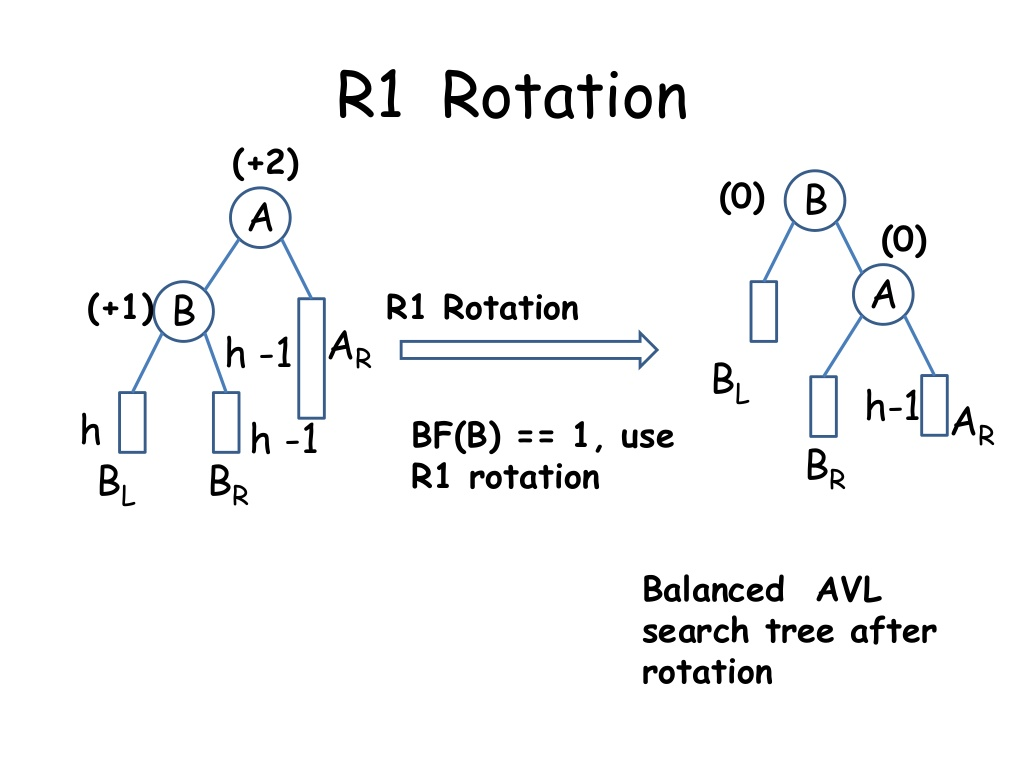
\includegraphics[width=250pt]{imagens/exemplo_remocao6.png}
  \label{fig_exemplo_remocao6}
\end{figure}
\end{frame}

%------------------------------------------------

\begin{frame}{Remoção}{Exemplo}
\begin{figure}[!h]
  \centering
  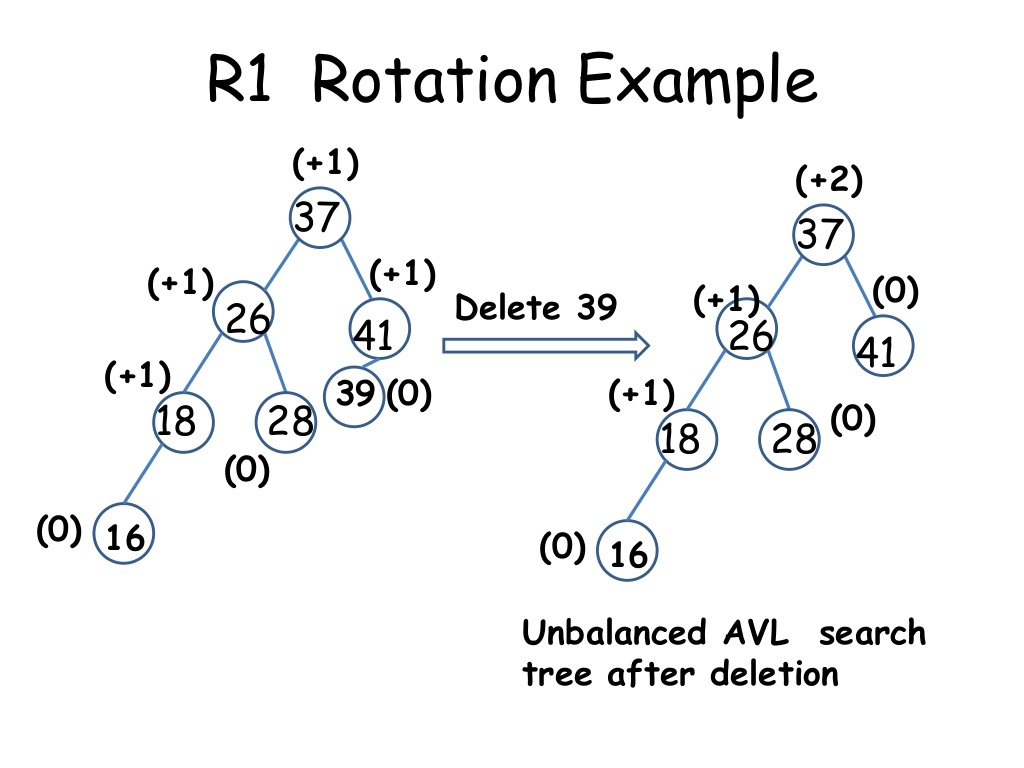
\includegraphics[width=250pt]{imagens/exemplo_remocao7.png}
  \label{fig_exemplo_remocao7}
\end{figure}
\end{frame}

%------------------------------------------------

\begin{frame}{Remoção}{Exemplo}
\begin{figure}[!h]
  \centering
  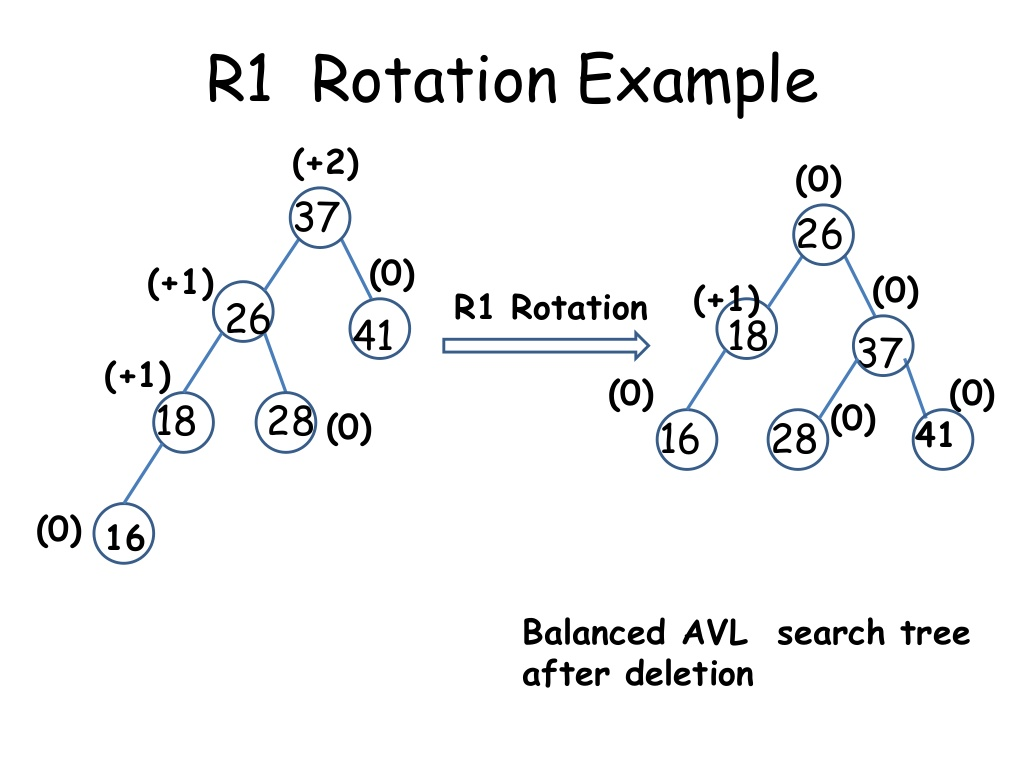
\includegraphics[width=250pt]{imagens/exemplo_remocao8.png}
  \label{fig_exemplo_remocao8}
\end{figure}
\end{frame}

%------------------------------------------------

\begin{frame}{Remoção}{Exemplo}
\begin{figure}[!h]
  \centering
  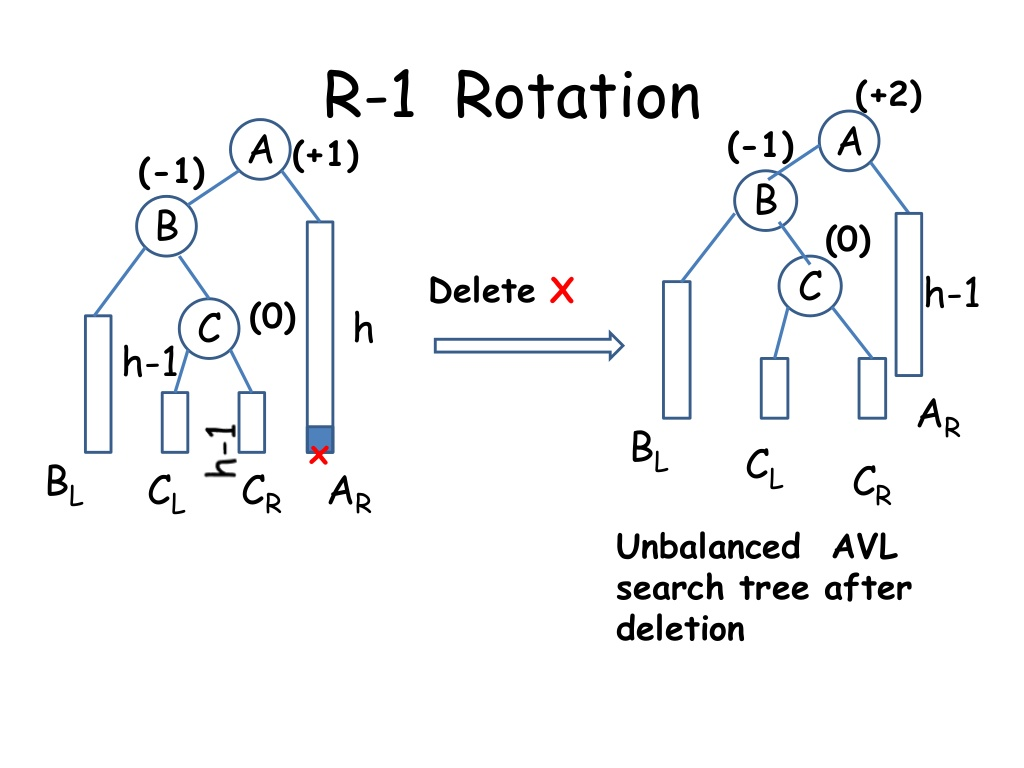
\includegraphics[width=250pt]{imagens/exemplo_remocao9.png}
  \label{fig_exemplo_remocao9}
\end{figure}
\end{frame}

%------------------------------------------------

\begin{frame}{Remoção}{Exemplo}
\begin{figure}[!h]
  \centering
  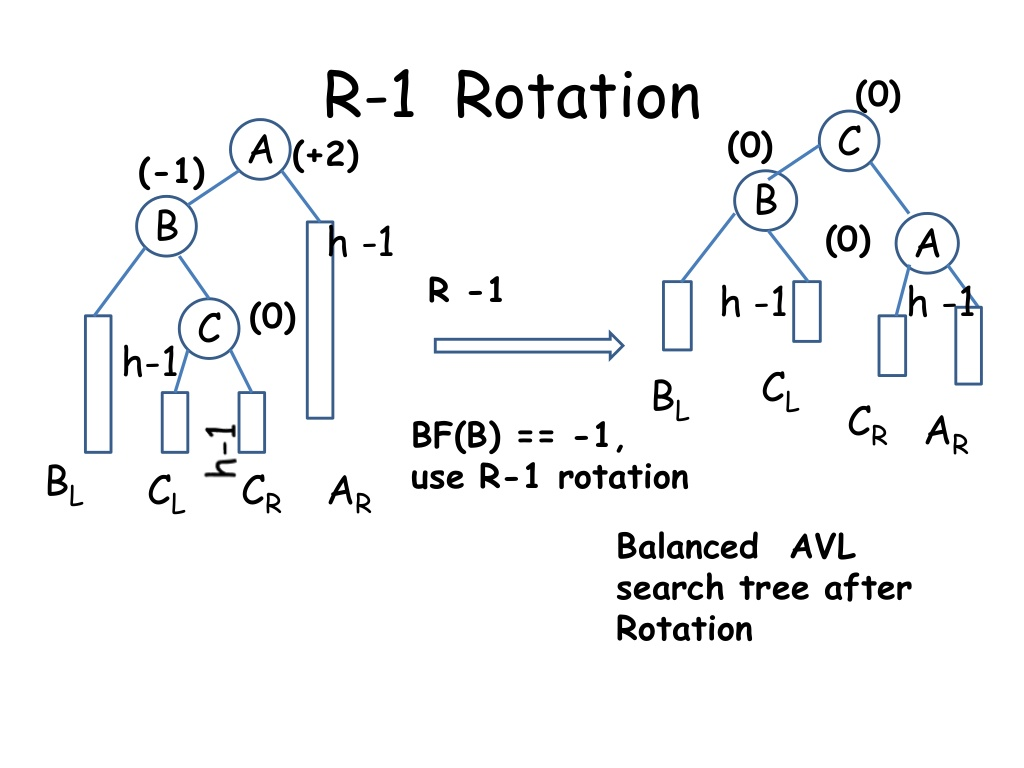
\includegraphics[width=250pt]{imagens/exemplo_remocao10.png}
  \label{fig_exemplo_remocao10}
\end{figure}
\end{frame}

%------------------------------------------------

\begin{frame}{Remoção}{Exemplo}
\begin{figure}[!h]
  \centering
  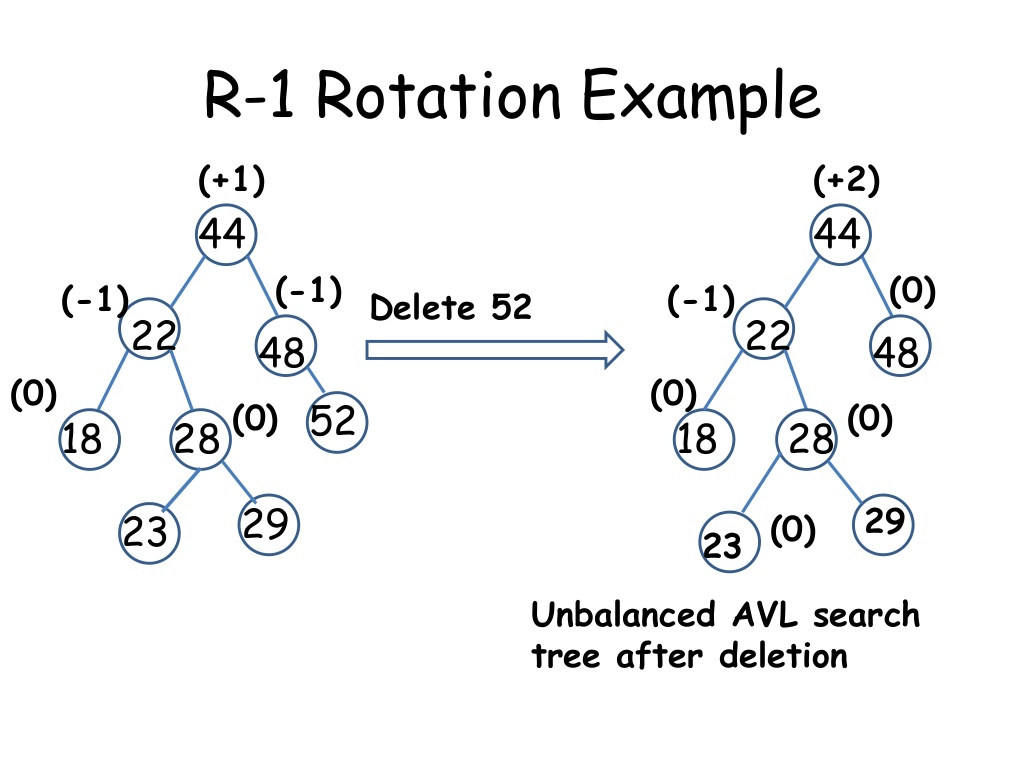
\includegraphics[width=250pt]{imagens/exemplo_remocao11.png}
  \label{fig_exemplo_remocao11}
\end{figure}
\end{frame}
%------------------------------------------------

\begin{frame}{Remoção}{Exemplo}
\begin{figure}[!h]
  \centering
  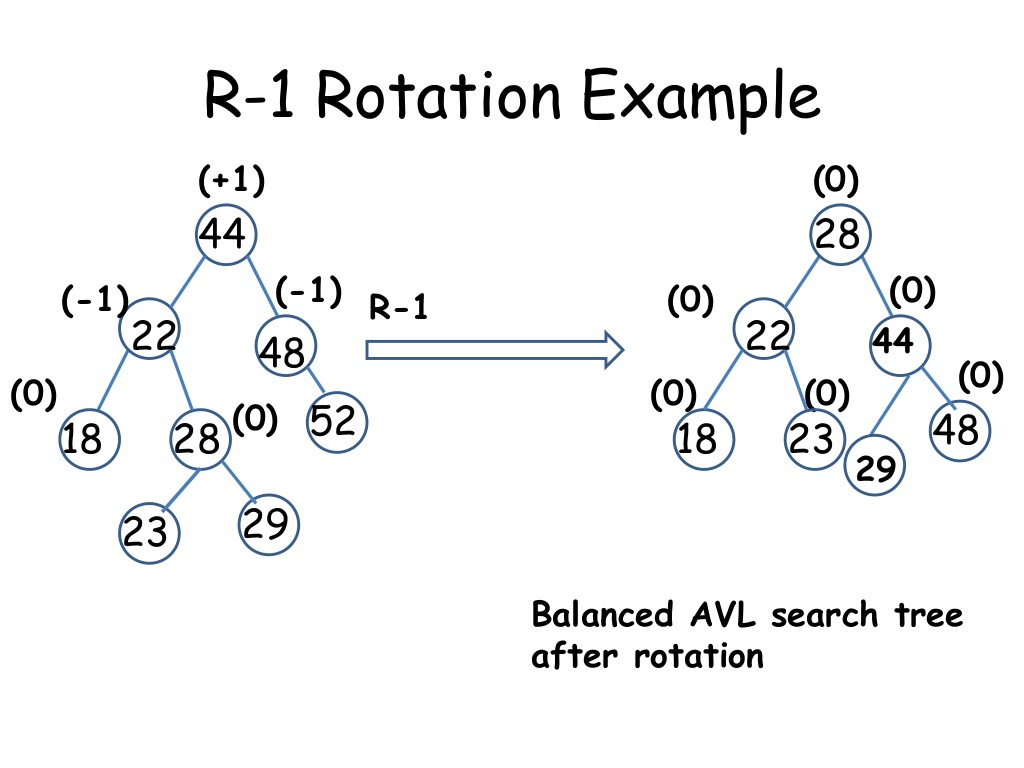
\includegraphics[width=250pt]{imagens/exemplo_remocao12.png}
  \label{fig_exemplo_remocao12}
\end{figure}
\end{frame}

%------------------------------------------------

\begin{frame}{Remoção}{Exemplo}
\begin{figure}[!h]
  \centering
  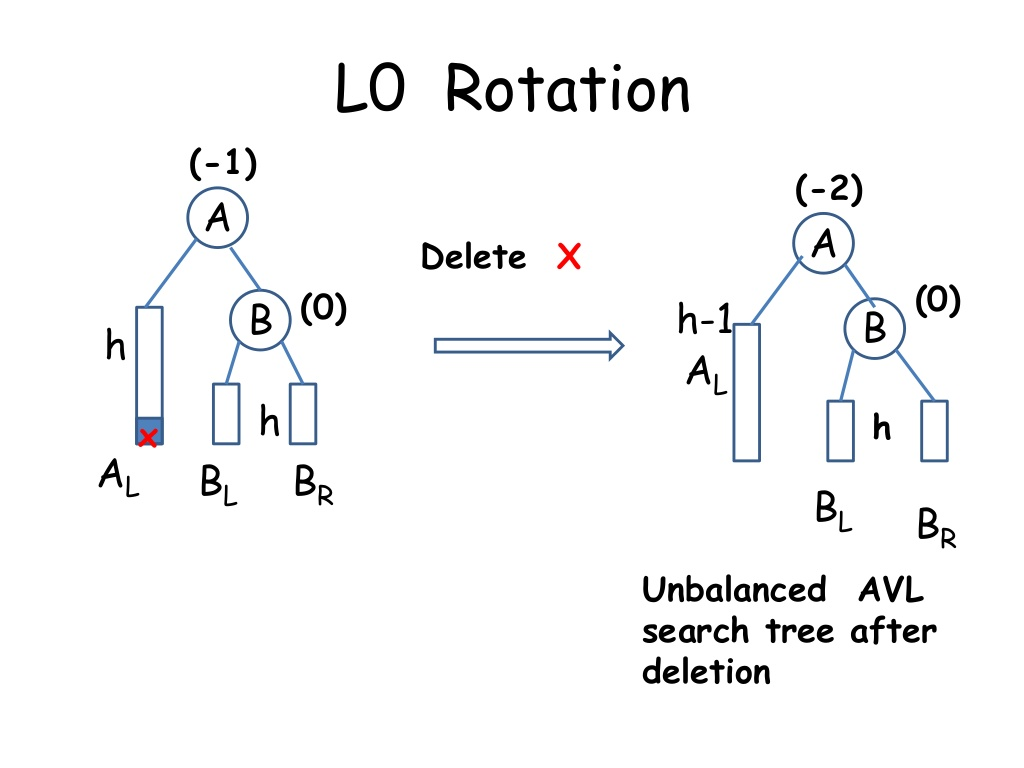
\includegraphics[width=250pt]{imagens/exemplo_remocao13.png}
  \label{fig_exemplo_remocao13}
\end{figure}
\end{frame}

%------------------------------------------------

\begin{frame}{Remoção}{Exemplo}
\begin{figure}[!h]
  \centering
  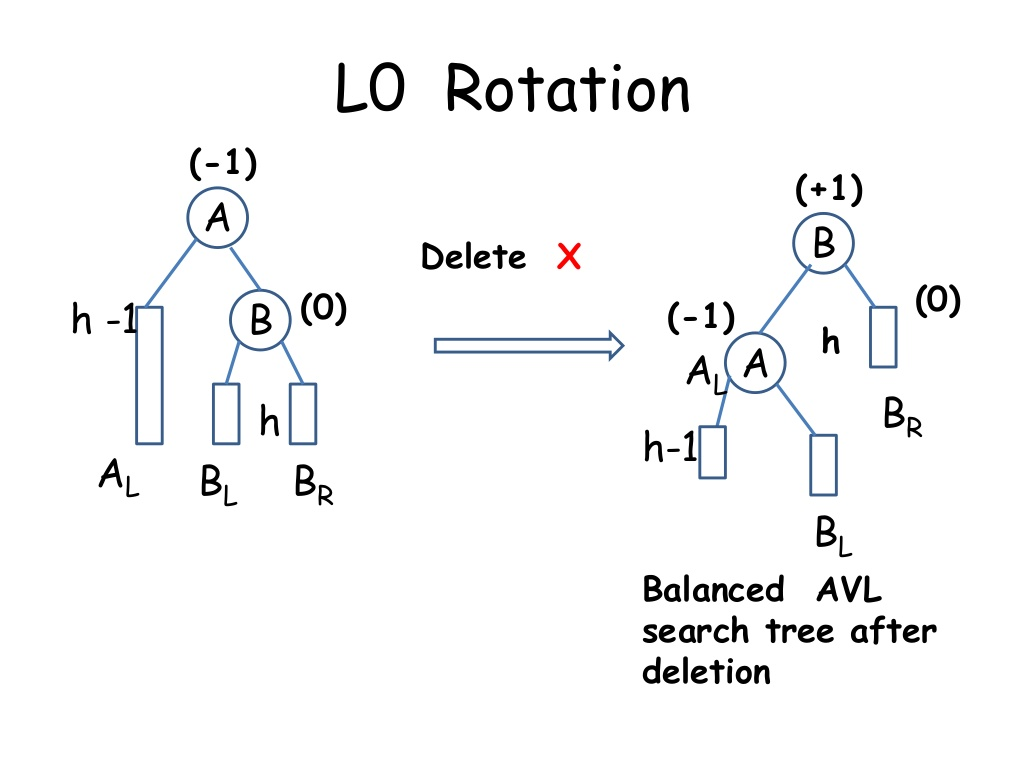
\includegraphics[width=250pt]{imagens/exemplo_remocao14.png}
  \label{fig_exemplo_remocao14}
\end{figure}
\end{frame}

%------------------------------------------------

\begin{frame}{Remoção}{Exemplo}
\begin{figure}[!h]
  \centering
  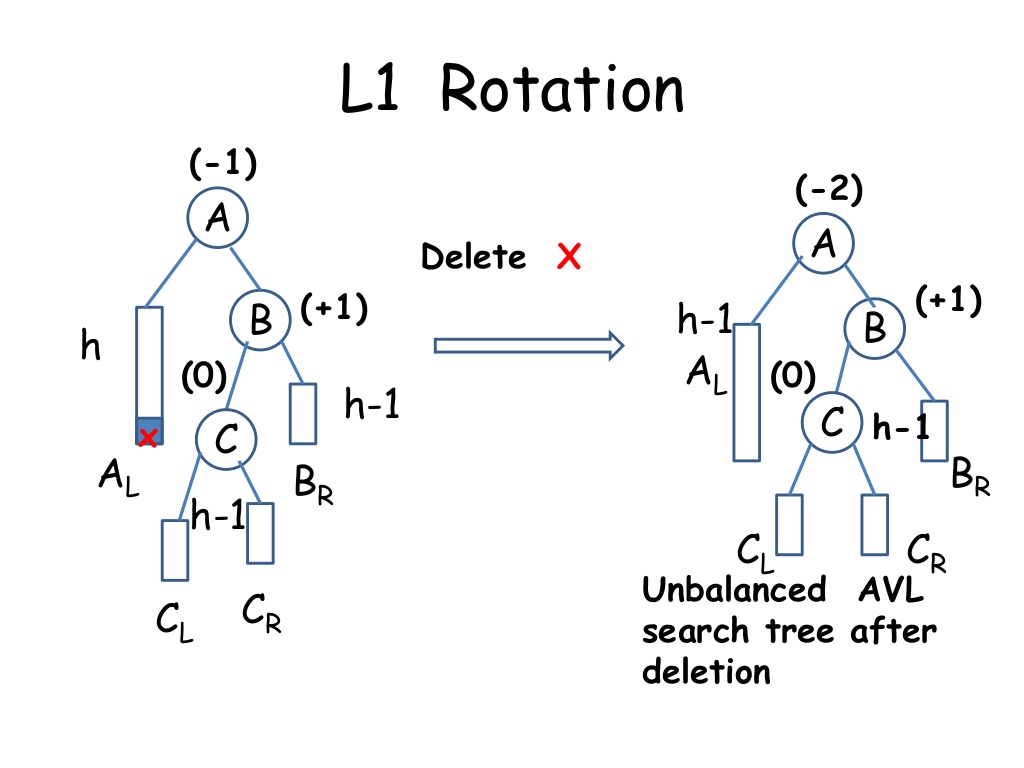
\includegraphics[width=250pt]{imagens/exemplo_remocao15.png}
  \label{fig_exemplo_remocao15}
\end{figure}
\end{frame}

%------------------------------------------------

\begin{frame}{Remoção}{Exemplo}
\begin{figure}[!h]
  \centering
  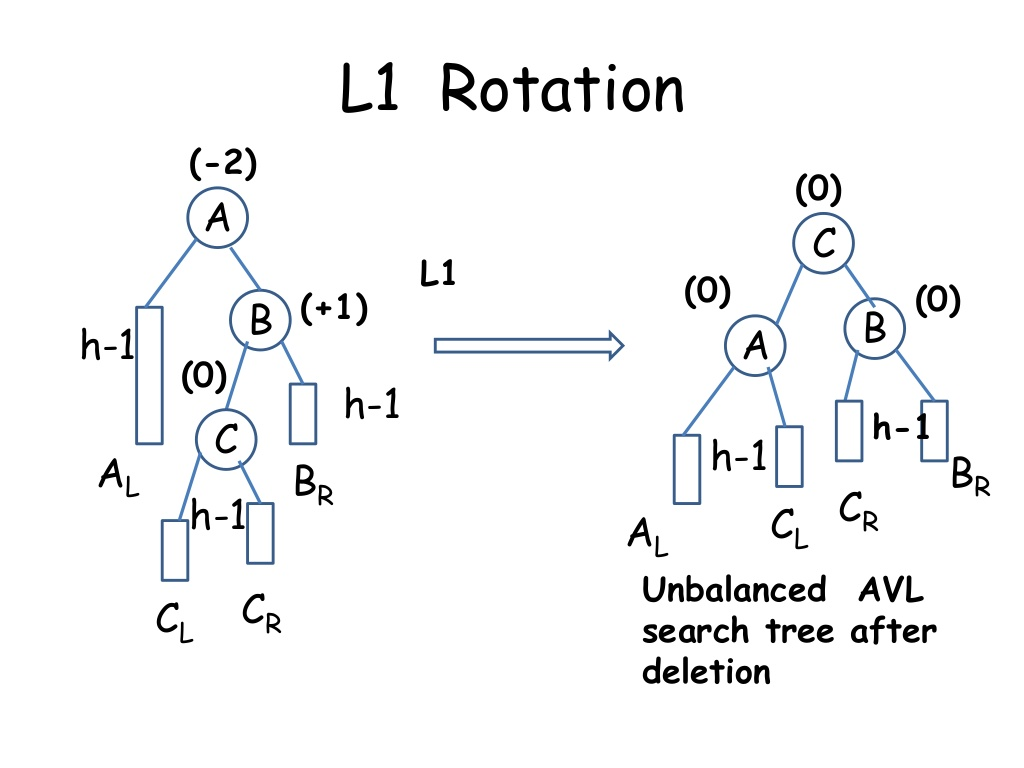
\includegraphics[width=250pt]{imagens/exemplo_remocao16.png}
  \label{fig_exemplo_remocao16}
\end{figure}
\end{frame}

%------------------------------------------------

\begin{frame}{Remoção}{Exemplo}
\begin{figure}[!h]
  \centering
  \includegraphics[width=250pt]{imagens/exemplo_remocao17.png}
  \label{fig_exemplo_remocao17}
\end{figure}
\end{frame}

%------------------------------------------------

\begin{frame}{Remoção}{Exemplo}
\begin{figure}[!h]
  \centering
  \includegraphics[width=250pt]{imagens/exemplo_remocao18.png}
  \label{fig_exemplo_remocao18}
\end{figure}
\end{frame}

%------------------------------------------------
%
%\begin{frame}
%\Huge{\centerline{Dúvidas?}}
%
%\begin{figure}[!h]
%  \centering
%  \includegraphics[width=100pt]{imagens/duvidas.jpg}
%  \label{fig_fim}
%\end{figure}
%\end{frame}

%----------------------------------------------------------------------------------------

\begin{frame}{Referências}{Bibliografia Básica}
\begin{itemize}
\item Livro Base
\begin{itemize}
\item \bibliographystyle{abnt-alf}
\bibliography{referencias}
\end{itemize}
\item Material Complementar
\begin{itemize}
\item \href{https://programacaodescomplicada.wordpress.com/complementar/}{Código-fonte e listas de exercícios - Material disponível on-line}.
\end{itemize}
\item Vídeo-aulas
\begin{itemize}
\item \href{https://www.youtube.com/watch?v=Au-6c55J90c&index=78&list=PL8iN9FQ7_jt6H5m4Gm0H89sybzR9yaaka}{Canal do youtube do prof. André Backes.}
\item \href{https://www.youtube.com/watch?v=YkF76cOgtMQ&t=92s}{Vídeo-aula: Estrutura de dados - Univesp}
\end{itemize}
\item Animações
\begin{itemize}
\item \href{https://www.cs.usfca.edu/~galles/visualization/AVLtree.html}{Árvore AVL - prof. David Galles - USFCA}
\end{itemize}
\end{itemize}
\end{frame}

%----------------------------------------------------------------------------------------

\end{document} 